\documentclass[11pt, a4paper]{book}
\usepackage[utf8]{inputenc}
\usepackage{multirow}
\usepackage{graphicx}
\graphicspath{ {../images} }

\usepackage[T1]{fontenc}


\usepackage[spanish, es-lcroman]{babel}
\usepackage{amsmath}
\usepackage{amsthm}
\usepackage{amsfonts}
\usepackage{amssymb}
\usepackage{titlesec}
\usepackage{enumerate}
\usepackage{enumitem}
\usepackage{graphicx}
\usepackage{mathtools}
\usepackage{array}
\usepackage{float}
\usepackage{pgfplots}
\usepackage{parskip}
\usetikzlibrary{fit,backgrounds}
\usepackage[]{hyperref}

\usepackage{changepage}
\usepackage{tikz}
\usepackage{nameref}

\usepackage[a4paper]{geometry}
\geometry{top=2.5cm, bottom=2.5cm, left=2.75cm, right=2.75cm}
\pagenumbering{arabic}

\usepackage{fancyhdr}
\pagestyle{fancy} 
\fancypagestyle{plain}{\fancyhf{}\fancyhead[L]{\quad\leftmark}\fancyhead[R]{\thepage}} 

\fancyhf{} % Limpia los encabezados y pies de página

% Configuración del encabezado
\fancyhead[L]{\quad\leftmark} % Muestra número de sección
\fancyhead[R]{\thepage}         % Número de página a la derecha





\title{Título y portada chula}

\begin{document}
	\maketitle
	
	\tableofcontents
	\newpage
	\thispagestyle{empty}
	
	\chapter{Documentación inicial}
	
	\section{Introducción}
	\textbf{El Problema del Viajante} es una agencia de viajes ficticia en la que se ofrecerán todo tipo de servicios relacionados con la planificación y la gestión de viajes, incluyendo transporte, alojamiento, lugares de interés para visitar, ocio, restauración, etc.
	
	\textcolor{red}{------------ Hay que mejorar la intro ---------}
	\textcolor{red}{Poner en algún lado que nosotros no hacemos las reservas como tal, solo lo ponemos bonito y redirigimos a otros lugares donde sí se puede reservar}
	
	El proyecto puede encontrarse en \href{https://github.com/PedroVidalVillalba/DAW_P1}{https://github.com/PedroVidalVillalba/DAW\_P1}, donde se encuentra también la última versión estable de este mismo documento y de la página web.
	
	
	Se han utilizado como inspiración diferentes páginas web de reserva de viajes, en especial \href{https://experiencetravelgroup.com}{Experience travel group}, aunque también se han consultado:
	\begin{itemize}
		\item \href{https://booking.com}{Booking}
		\item \href{https://tripadvisor.es}{Tripadvisor}
		\item \href{https://skyscanner.es}{Skyscanner}
		\item \href{https://calendar.google.com/calendar/u/0/r}{Google Calendar}
	\end{itemize}
	
	 En estas páginas se puede comprobar que es habitual ofrecer una experiencia lo más completa posible respecto a la organización desde el mismo lugar el transporte y alojamiento. Pero hemos echado en falta que ninguna tenga aspectos más relacionados con la planificación en el propio viaje, como lugares de interés o restaurantes, y que incluso se pueda acceder a la reserva desde la propia página, de forma que se cree un itinerario. Además, ya no sería necesario acceder a otro lugar para indicar en el calendario las fechas indicadas, sino que ya se mostrarían en la propia página, y este calendario podría sincronizarse con el de la cuenta de Google, u otros semejantes.
	
	
	
	\section{Inventario de contenido}
	Inicialmente se ha realizado una tormenta de ideas, en la que se ha reflexionado sobre el tema escogido, y su contenido, audiencia, elementos visuales atractivos para el usuario, etc. Los contenidos iniciales de la tormenta de ideas se pueden consultar en el \nameref{chap:anexo1}. Los elementos principales sobre los que se estructura la aplicación son:
	
	\begin{itemize}
		\item Reserva de hoteles, aviones y otros medios de transporte. En general, cómo ir desde el lugar donde vive el usuario hasta su destino.
		\item Lugares de interés para visitar, con fotos, su web, ubicación, etc. 
		\item Lugares de ocio, restauración, y otro tipo de tiendas conocidas en la zona.
		\item Calendario con planificación del viaje, desde el que acceder a la información sobre el medio de transporte elegido, alojamiento, etc. y que permita organizar los lugares de visita de cada día.
		\item Lista de lugares y tiendas favoritos, junto a un mapa integrado en donde aparezcan destacados.
		\item Experiencias exclusivas, con planificaciones de viajes realizadas previamente por expertos.
	\end{itemize} 
	
	Después de analizar los elementos obtenidos, filtrarlos y establecer relaciones entre sí, se ha llegado al siguiente inventario de contenido:

	\textcolor{red}{---------------Poner aquí el inventario de contenido. Hay que hacer un dibujín -------------------------}
	
	Otros elementos que también son relevantes para la justificación de la creación de la página web son:
	
	\begin{enumerate}
		\item \textbf{Audiencia}: un público genérico, ya que cada vez más personas viajan de forma relativamente habitual, y resulta de gran utilidad una página web desde la que poder gestionar todo el viaje.
		\item \textbf{Elementos visuales}: principalmente imágenes y vídeos de cada lugar, que deben llamar la atención del usuario sin ser excesivos, y también mapas. Se creará un logo generado con IA que sea característico de la empresa.
		\item \textbf{Financiación}: se podrían obtener beneficios a través de anuncios en la página. También se podría incluir un sistema de suscripción o mecenazgo con descuentos dentro de la página web, para clientes habituales.
	\end{enumerate}


	\section{Arquitectura de información}
	Una vez se dispone del inventario de contenido, se organizan estos elementos jerárquicamente en una arquitectura de la información, que dará una primera aproximación al número de páqinas que se necesitarán crear y al esquema de navegación que permite relacionarlas. 
	
	Se llega así, a alto nivel, a la siguiente estructura, en la que cada elemento principal tiene varias ramas:
	
	\begin{itemize}
		\item \textbf{Página principal}: presentación de la página que llame la atención, \textit{newsletter}, valoraciones, opiniones de expertos.
		\item \textbf{Descubre}: búsqueda de lugares visita, ocio, restauración etc., destinos de moda/recomendados, exploración, mapa de lugares favoritos.
		\item \textbf{Planifica}: calendario, consejos generales para viajes al extranjero, seguro de viajes, mecanismos de reserva con seguridad.
		\item \textbf{Reserva}: búsqueda de hoteles, búsqueda de aviones y otros medios de transporte, alquiler de coches, reserva de restaurantes, experiencias exclusivas.
		\item \textbf{About us}: quiénes somos, nuestra historia, qué nos diferencia, FAQ, redes sociales, nuestro sistema de puntuación, certificados de calidad, premios.
		\item \textbf{Otros}: términos de uso, política de cookies, política de privacidad.
	\end{itemize}

	\begin{figure} [H]
		\centering
		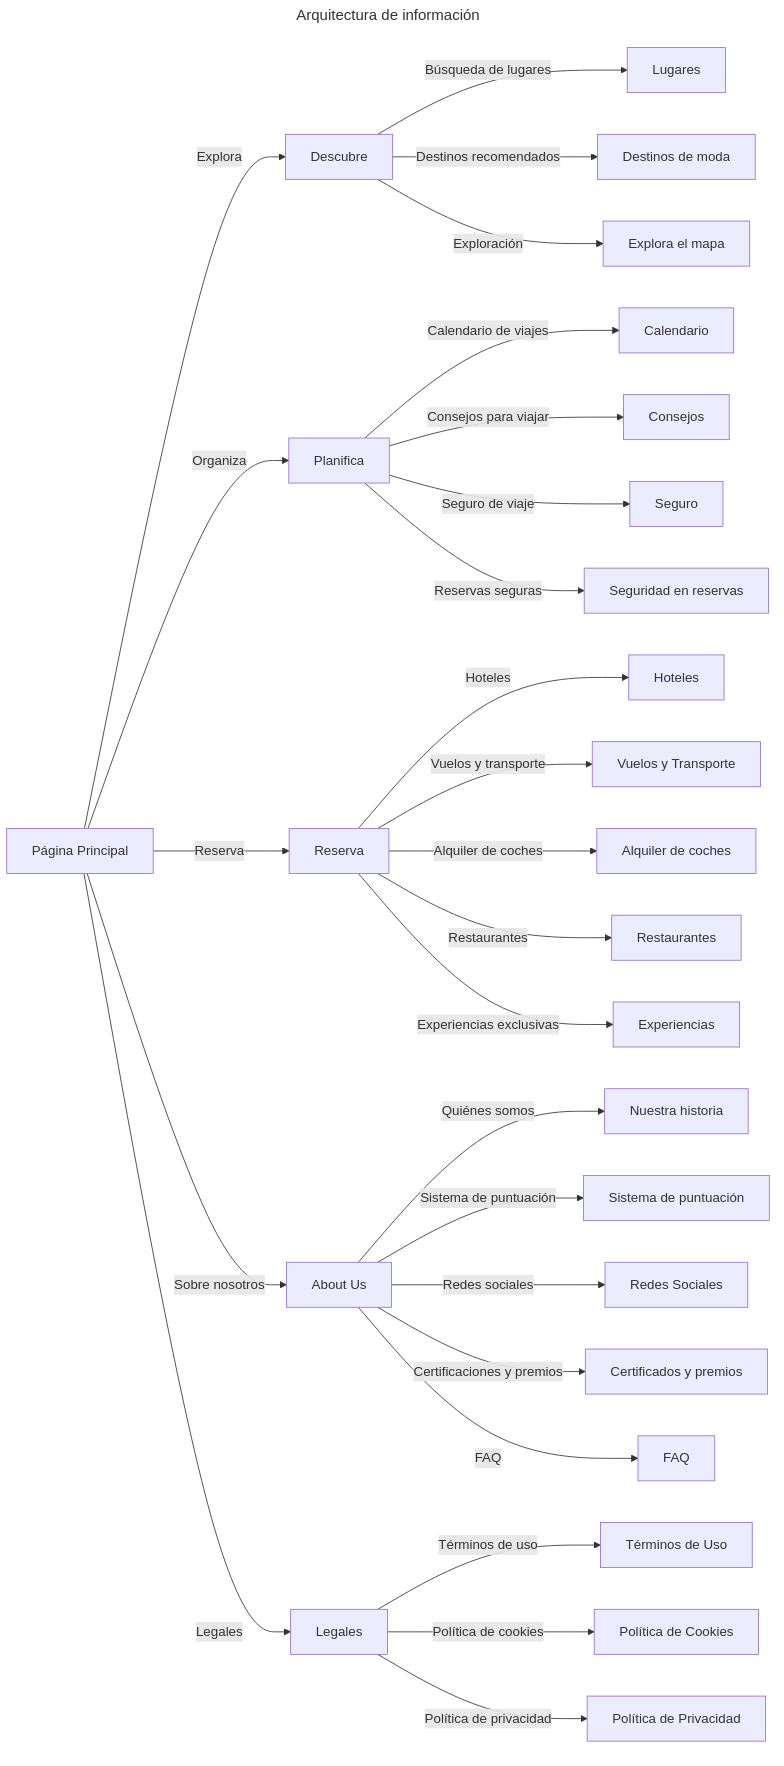
\includegraphics[height=0.85\textheight]{arquitectura_informacion.png}
		\caption{Arquitectura de información}
	\end{figure}
	
	
	
	\section{Mapa de navegación}
	El mapa de navegación plasma las relaciones jerárquicas recogidas por la arquitectura de la información y las organiza en páginas concretas que serán posteriormente implementables. Como se ve en la imagen, es similar a la arquitectura de información
	
	\begin{figure} [H]
		\centering
		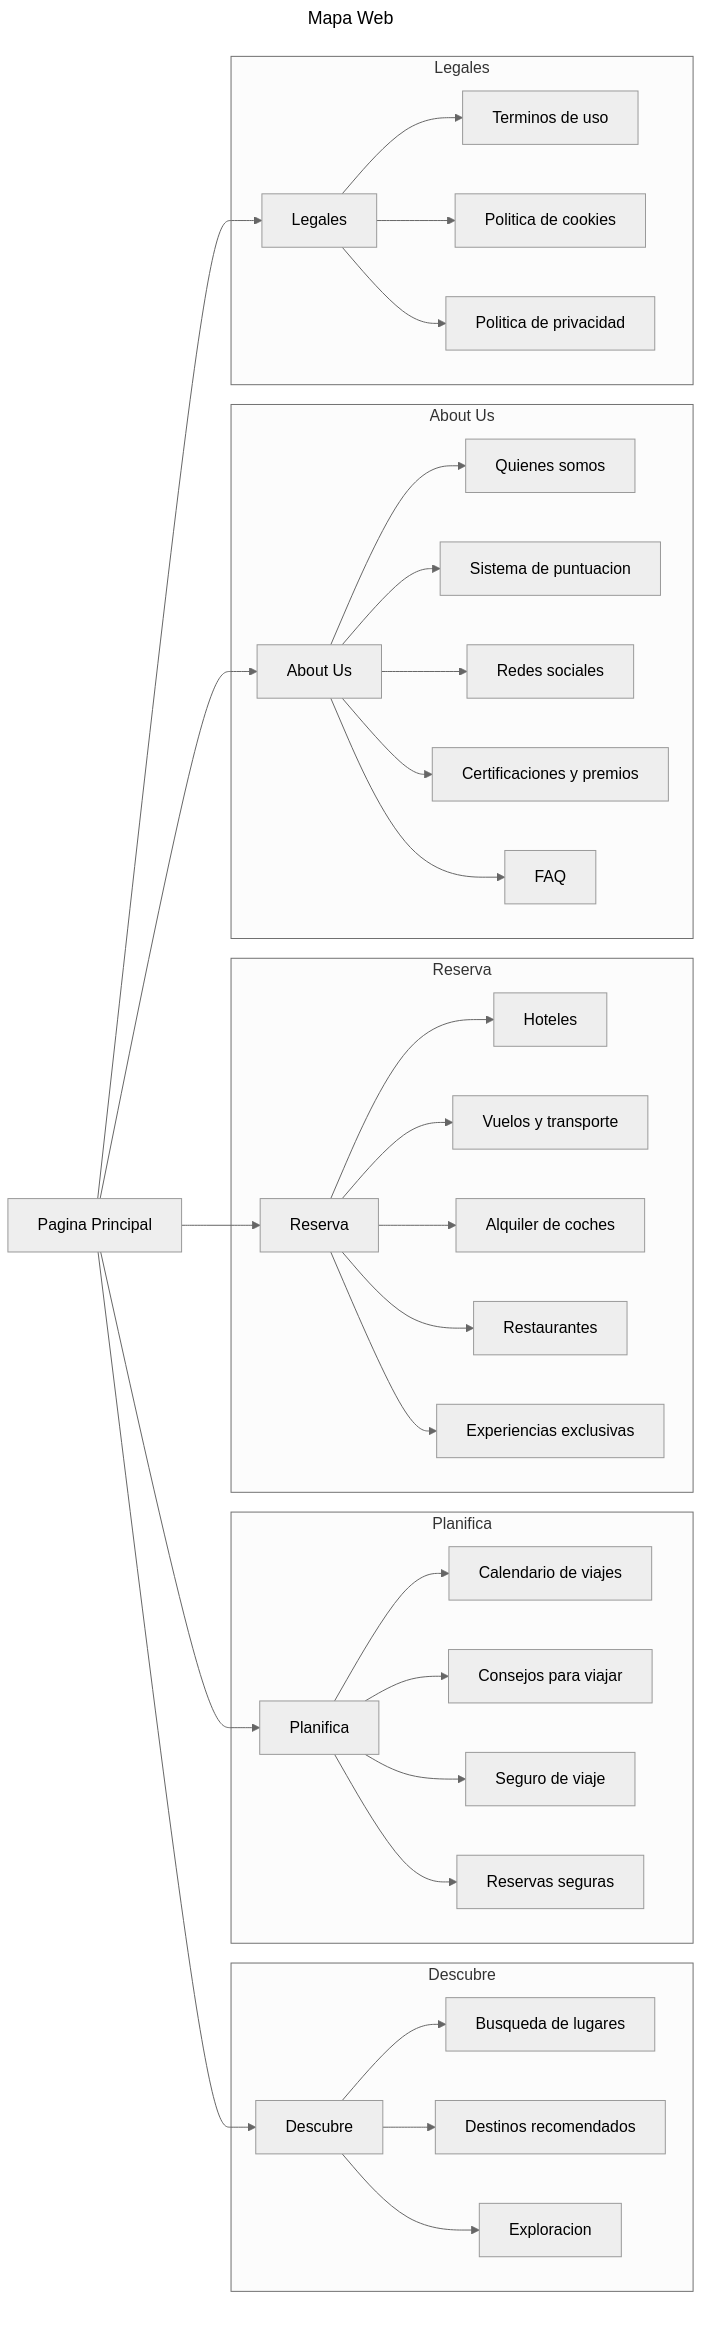
\includegraphics[height=0.85\textheight]{mapa_web.png}
		\caption{Mapa de navegación}
	\end{figure}
	
	
	
	\section{Interfaces}
	Con toda la información recogida, el siguiente paso es empezar a diseñar las interfaces, en las que se muestre un prototipo de la disposición, fuentes de texto, colores, imágenes y navegación en las diferentes páginas web. En este caso, se han realizado interfaces de las 5 páginas principales: la página principal, descubre, planifica, reserva y \textit{about us}. 
	
	Cada una incluye tres fases de desarrollo, una prototipo manual(\textit{sketch}) con las ideas básicas que conforman el sitio web, un esqueleto digital (\textit{wireframe}) centrado en la disposición de los elementos de acuerdo a proporciones adecuadas, y por último un diseño final (\textit{mockup}) de la interfaz, que muestra cómo debería ser la apariencia final de la página, incluyendo colores, fuentes de texto e imágenes adecuadas.
	
	\subsection{Prototipo manual}
	A continuación se muestran los bocetos de las interfaces realizadas a mano. Dado el carácter académico de este documento, se considera relevante incluirlas, a pesar de que en un entorno profesional su uso sería poco común. Se han realizado los prototipos para cinco ventanas, las cuales se comentan a continuación.
	
	\newpage % Mejor poner juntos imagen y descripción
	
	\begin{figure} [H]
		\centering
		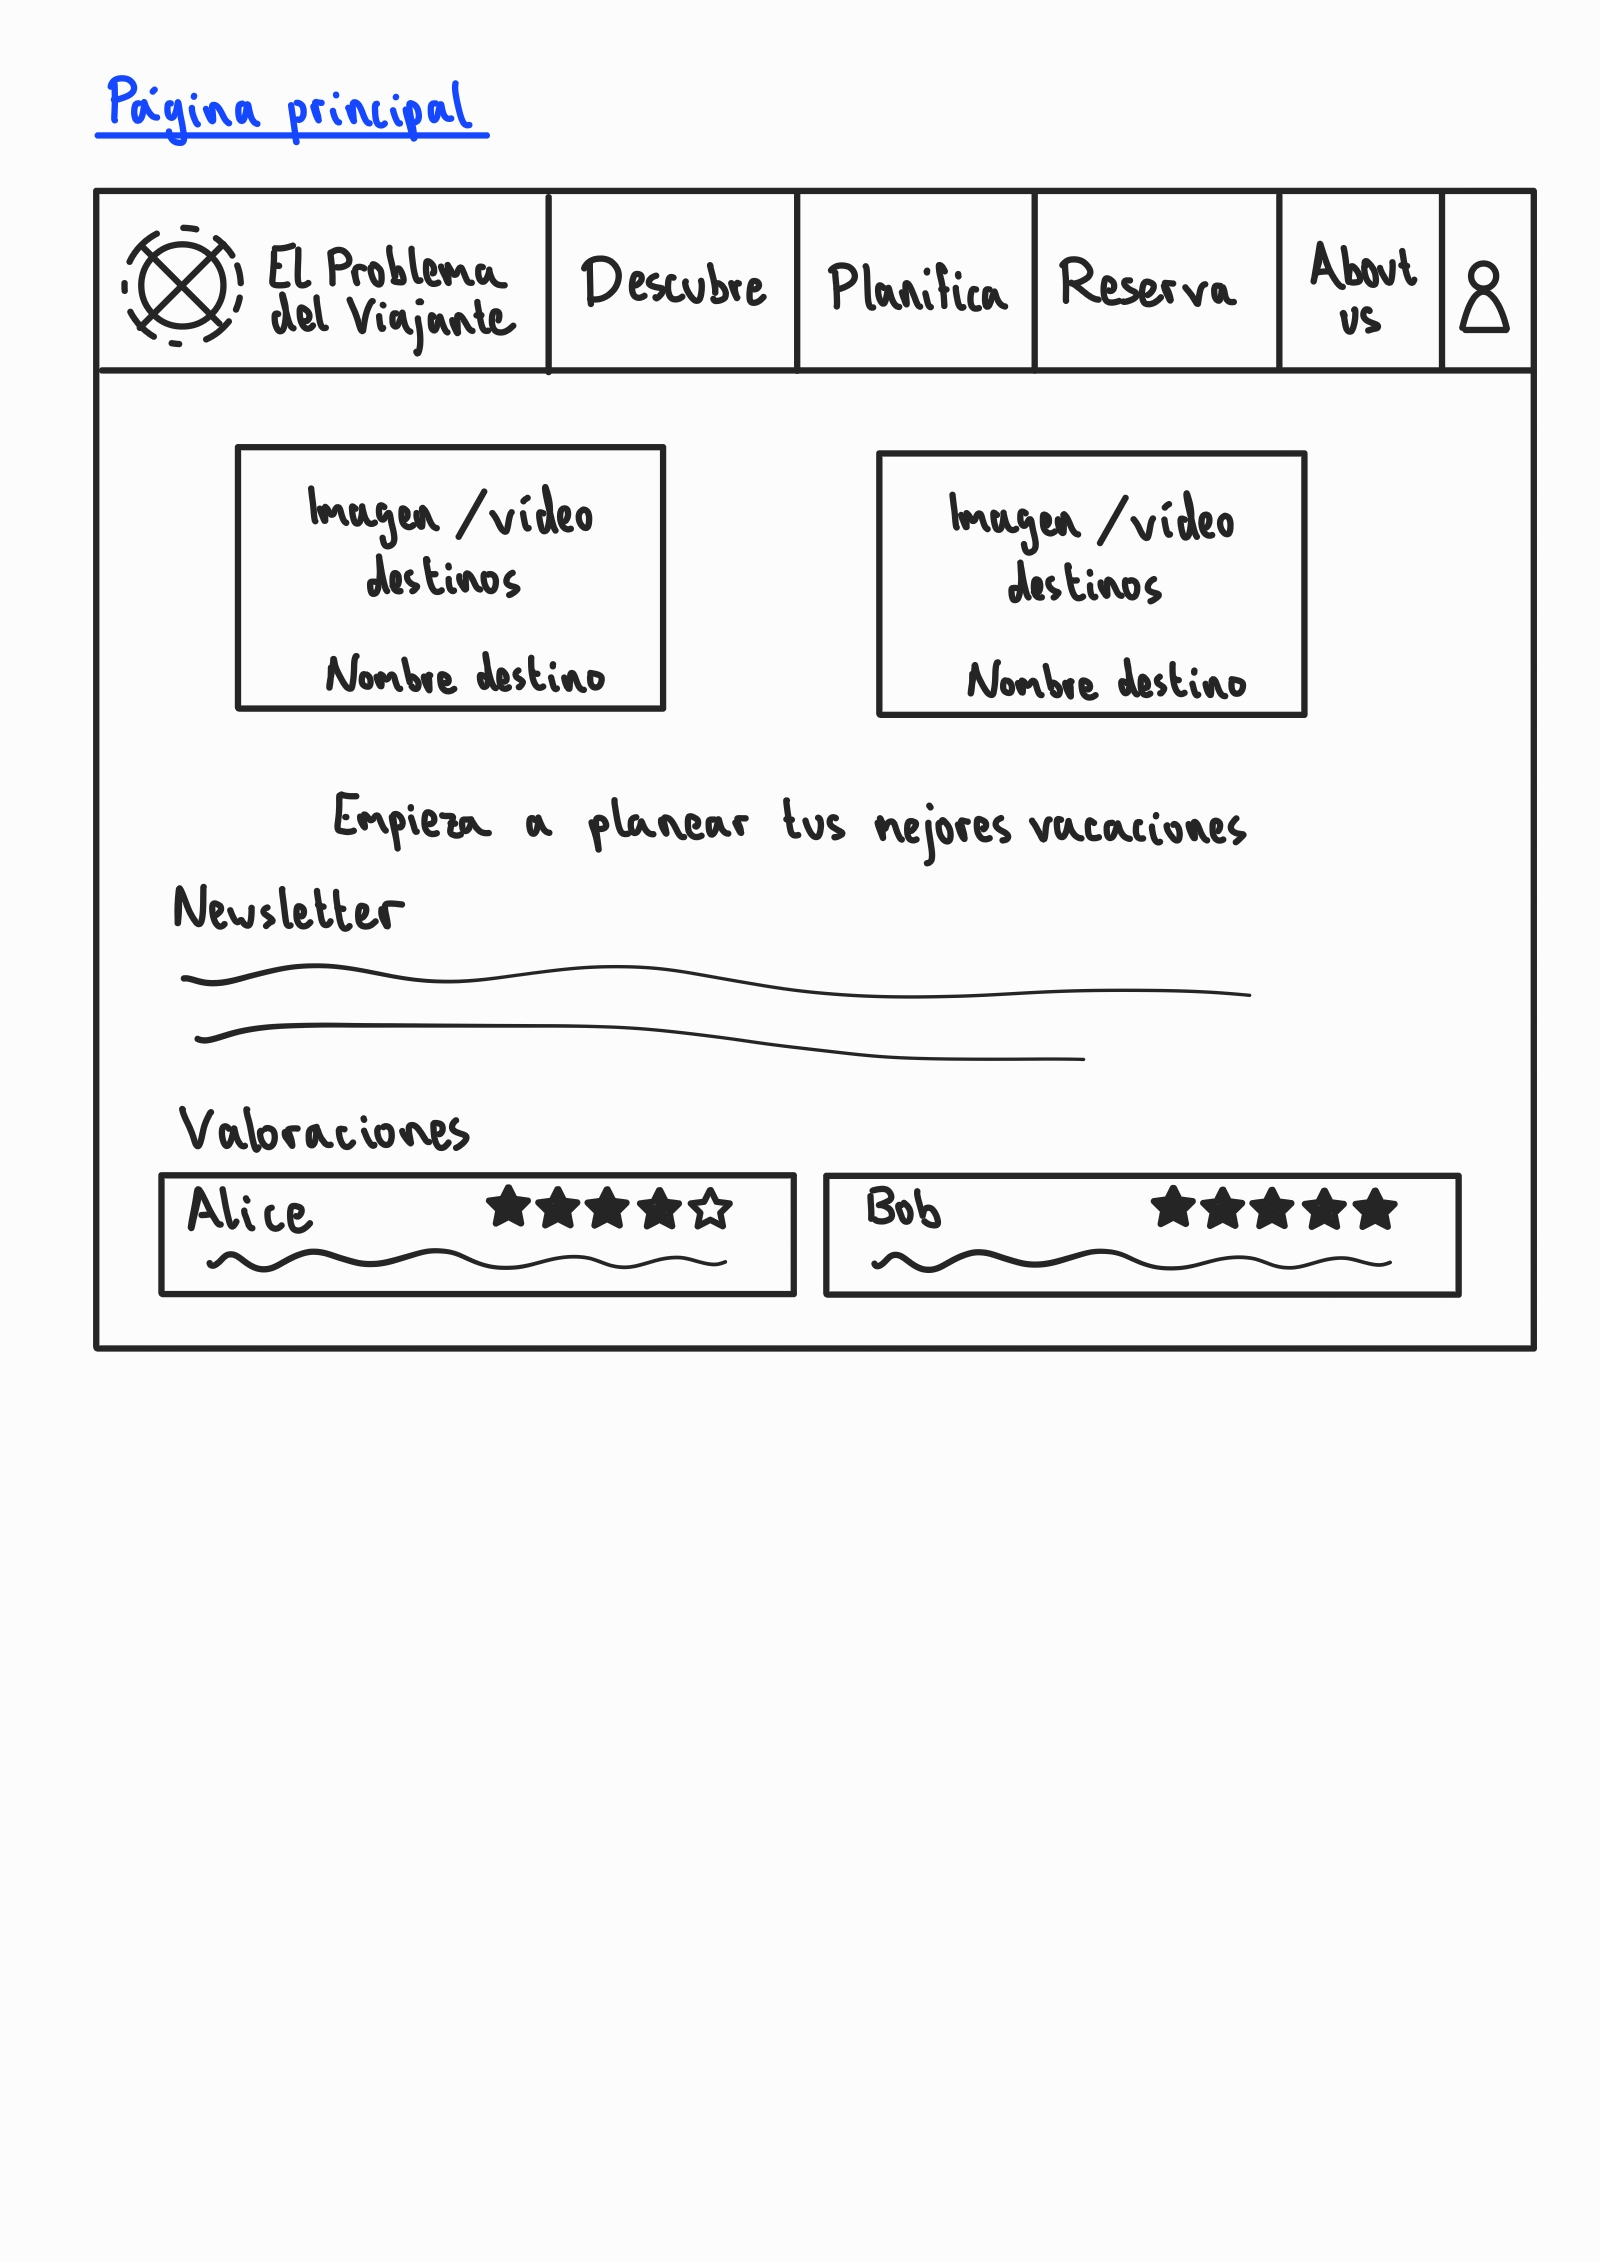
\includegraphics[width=\textwidth]{1-principal.jpg}
		\caption{Prototipo Página principal}
	\end{figure} 

	En esta figura se puede ver la \textbf{página principal} del sitio web. Aquí, se ve la barra de navegación global, que será común a todas las páginas, unos cuantos elementos visuales sobre algunos destinos destacados para captar la atención del visitante, un apartado de \textit{newsletter} con novedades importantes y una sección con valoraciones de clientes.
	
	Desde la barra de navegación, el usuario podrá registrarse por medio de correo electrónico para poder realizar valoraciones, que se guarden sus viajes, crear una planificación colaborativa y obtener mejores recomendaciones.
	
	\newpage
	
	\begin{figure} [H]
		\centering
		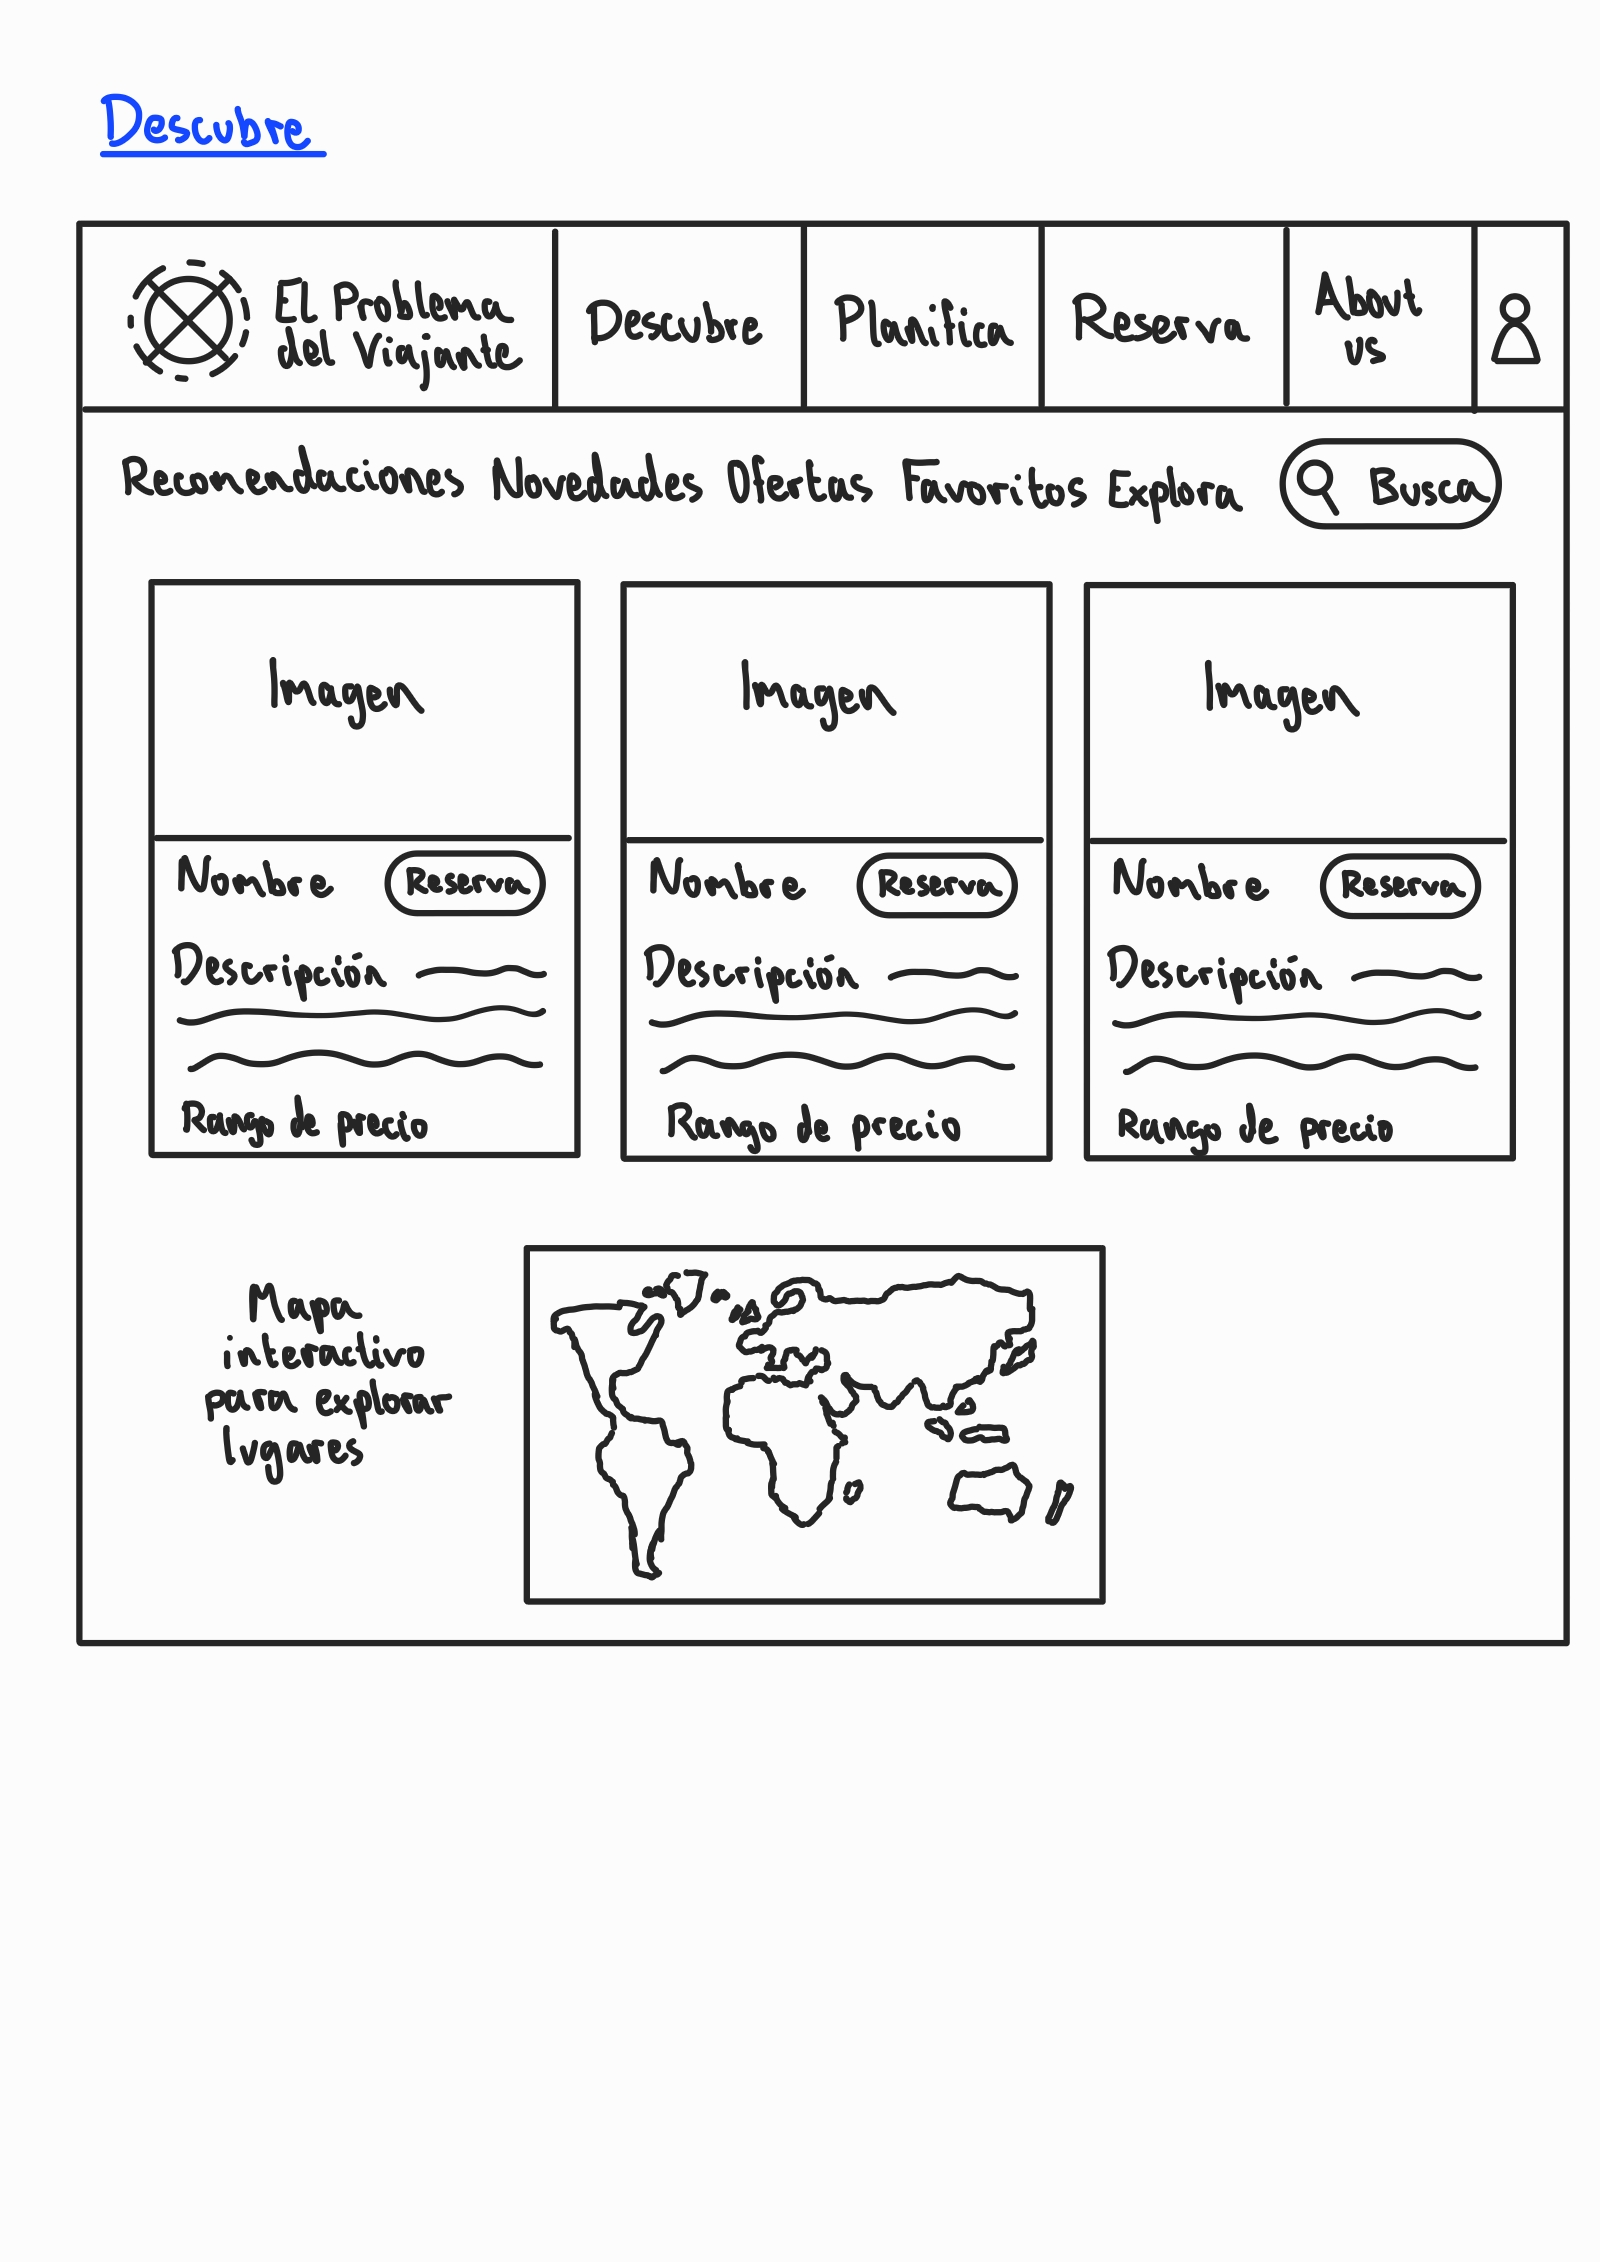
\includegraphics[width=\textwidth]{2-descubre.jpg}
		\caption{Prototipo Descubre}
	\end{figure} 

	En el apartado de \textbf{Descubre} se pretende que los clientes de la página que no tienen todavía claro cuál es el destino del viaje que quieren puedan explorar sus opciones. 
	
	Se ve, en primer lugar, una barra de navegación secundaria en la que aparecen diferentes subsecciones. En cada una de estas se presentarán destinos asociados al criterio empleado. En todas estas aparecerán diversos paquetes de viajes, mostrando imágenes y descripciones de los lugares a los que viajar. Asimismo, se incluye un mapa interactivo en el que aparecerán destacados los lugares mencionados en las tarjetas que aparecen en la página. Interactuando con este mapa, el cliente podrá, además, filtrar la búsqueda a un destino en concreto. Se incluyen además algunos destinos recomendados, consejos generales para la planificación de viajes y un apartado sobre la seguridad en las reservas.

	\newpage 
	
	\begin{figure} [H]
		\centering
		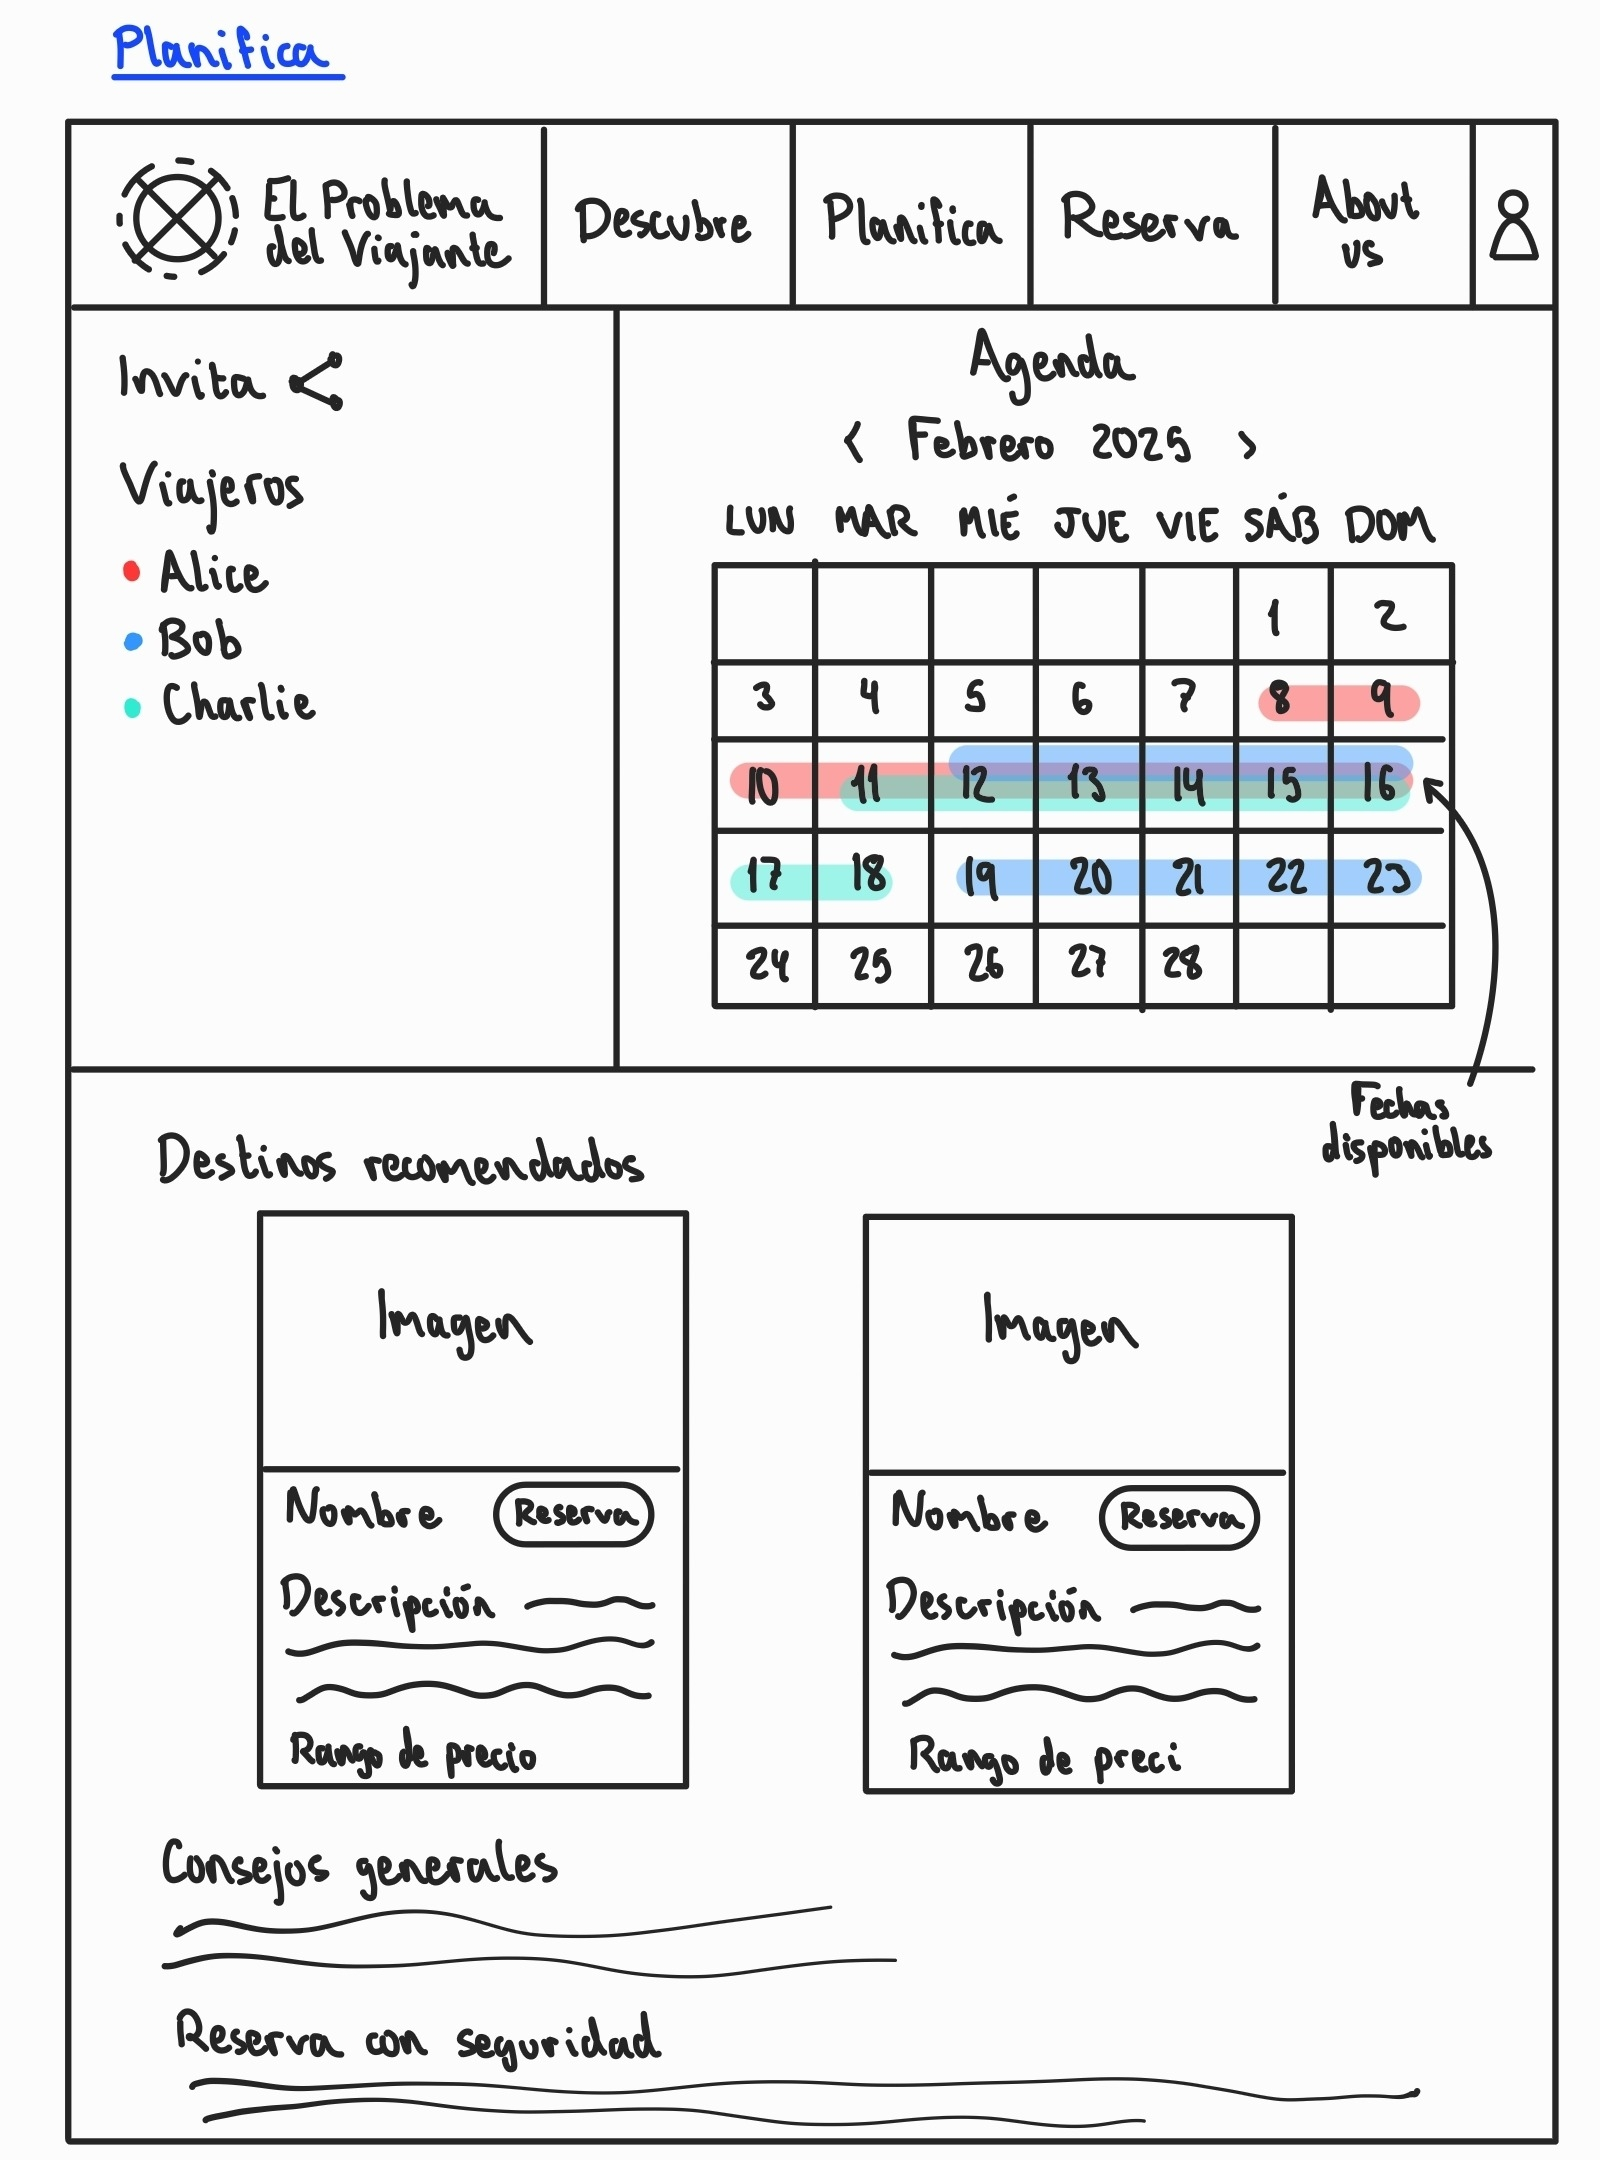
\includegraphics[width=\textwidth]{3-planifica.jpg}
		\caption{Prototipo Planifica}
	\end{figure} 

	En la sección de \textbf{Planifica}, el cliente podrá planificar su viaje con, posiblemente, otros usuarios. Así, están disponibles una columna en la que se puede invitar a otros viajeros y un calendario en el que cada uno de los participantes en un viaje puede marcar las fechas que tiene disponibles para una planificación más eficiente.

	\newpage
	
	\begin{figure} [H]
		\centering
		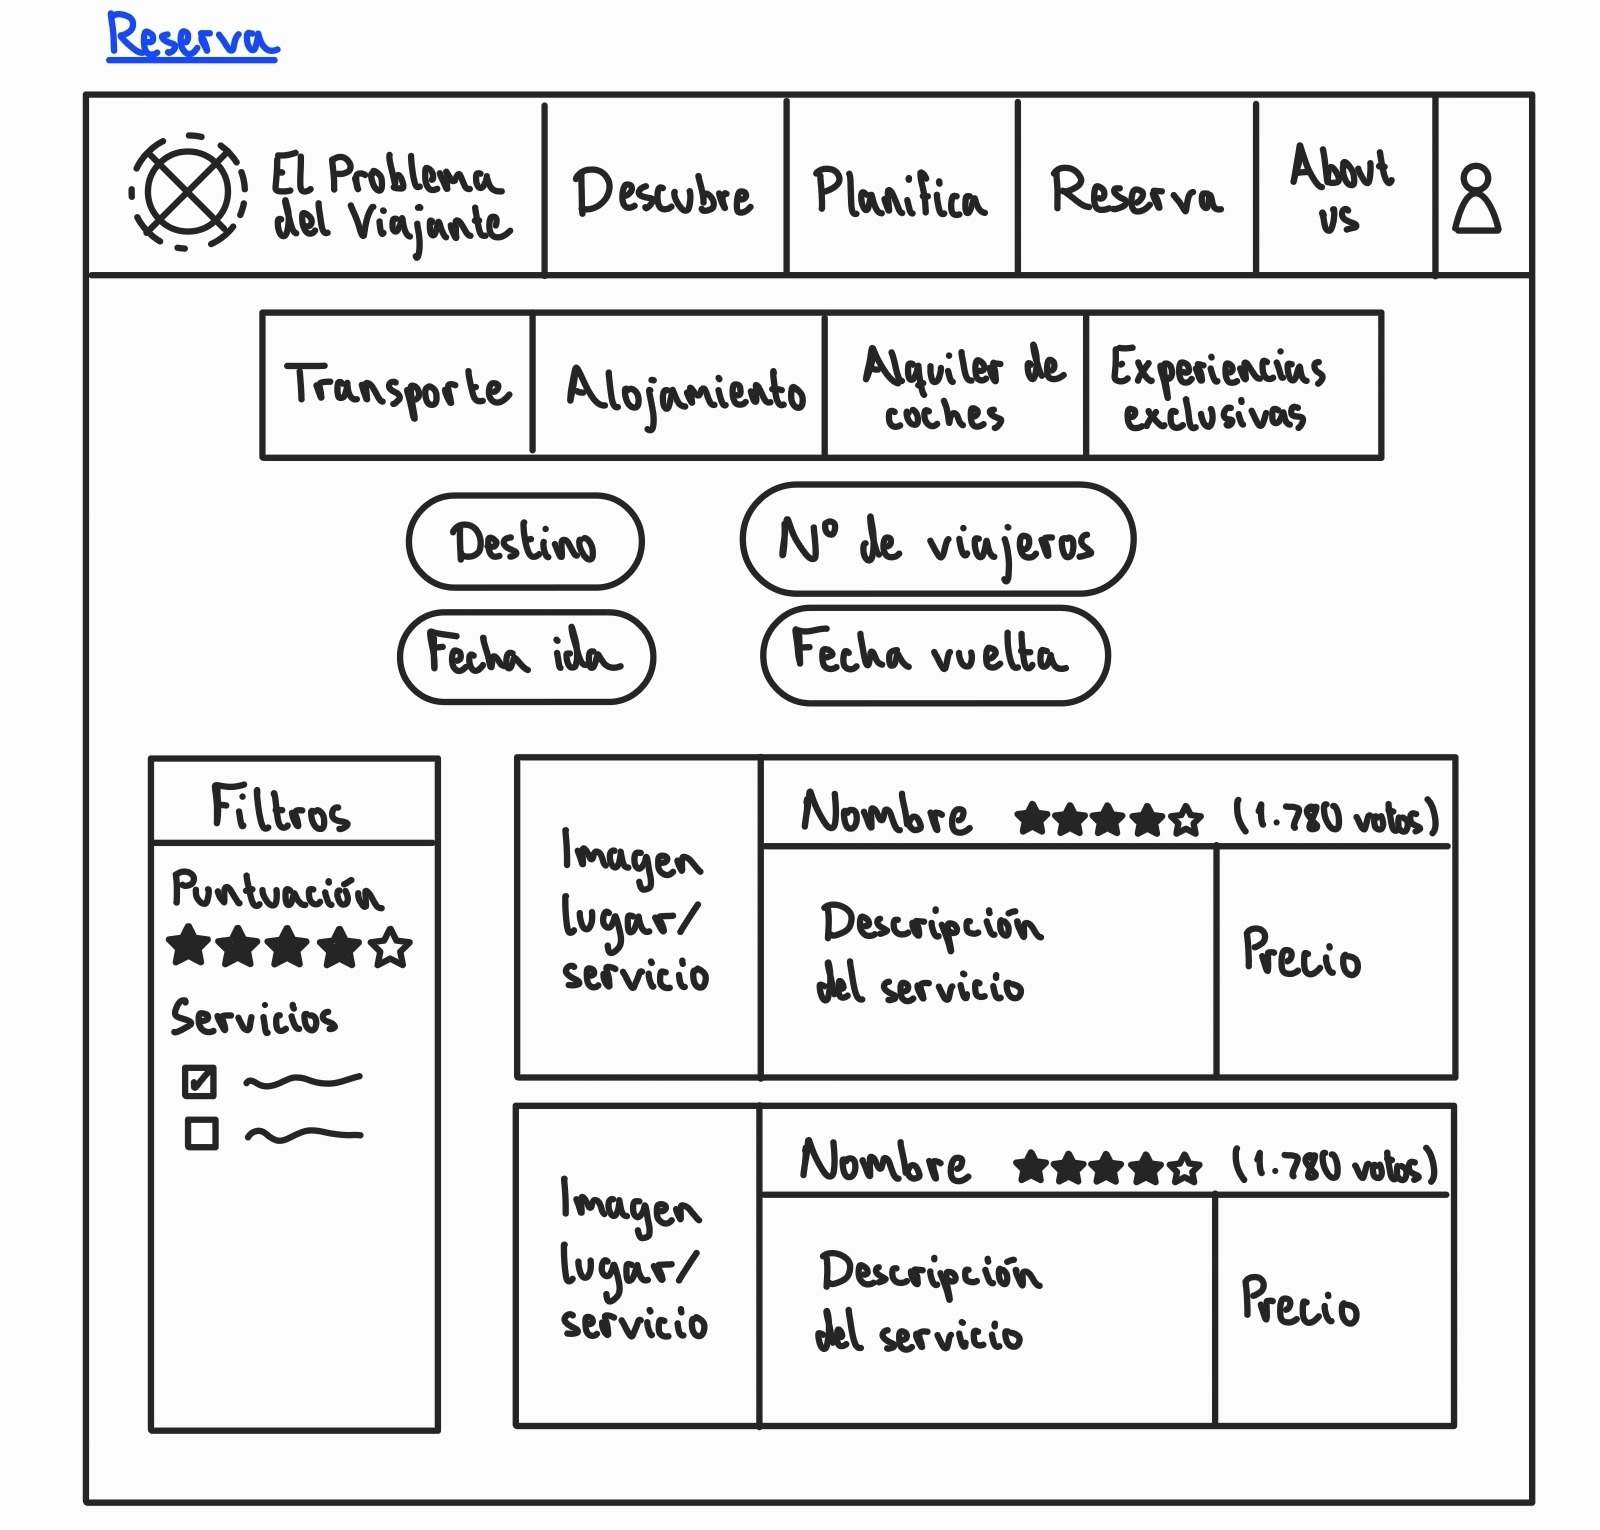
\includegraphics[width=\textwidth]{4-reserva.jpg}
		\caption{Prototipo Reserva}
	\end{figure} 

	En la página de \textbf{Reserva} el usuario podrá gestionar las reservas necesarias para su viaje. Estas incluyen el transporte hasta el lugar, alojamiento, alquiler de vehículos y otras experiencias exclusivas facilitadas por nuestro sitio web.
	
	Se incluye un filtro principal por destino, número de viajeros y fechas de ida y vuelta. Hay otros filtros secundarios que se podrán aplicar sobre la puntuación y el tipo de servicio. Una vez seleccionados estos campos, aparecerán los servicios recomendados por la web, con una imagen, su nombre, descripción y precio para que el usuario pueda gestionar su reserva.

	\newpage

	\begin{figure} [H]
		\centering
		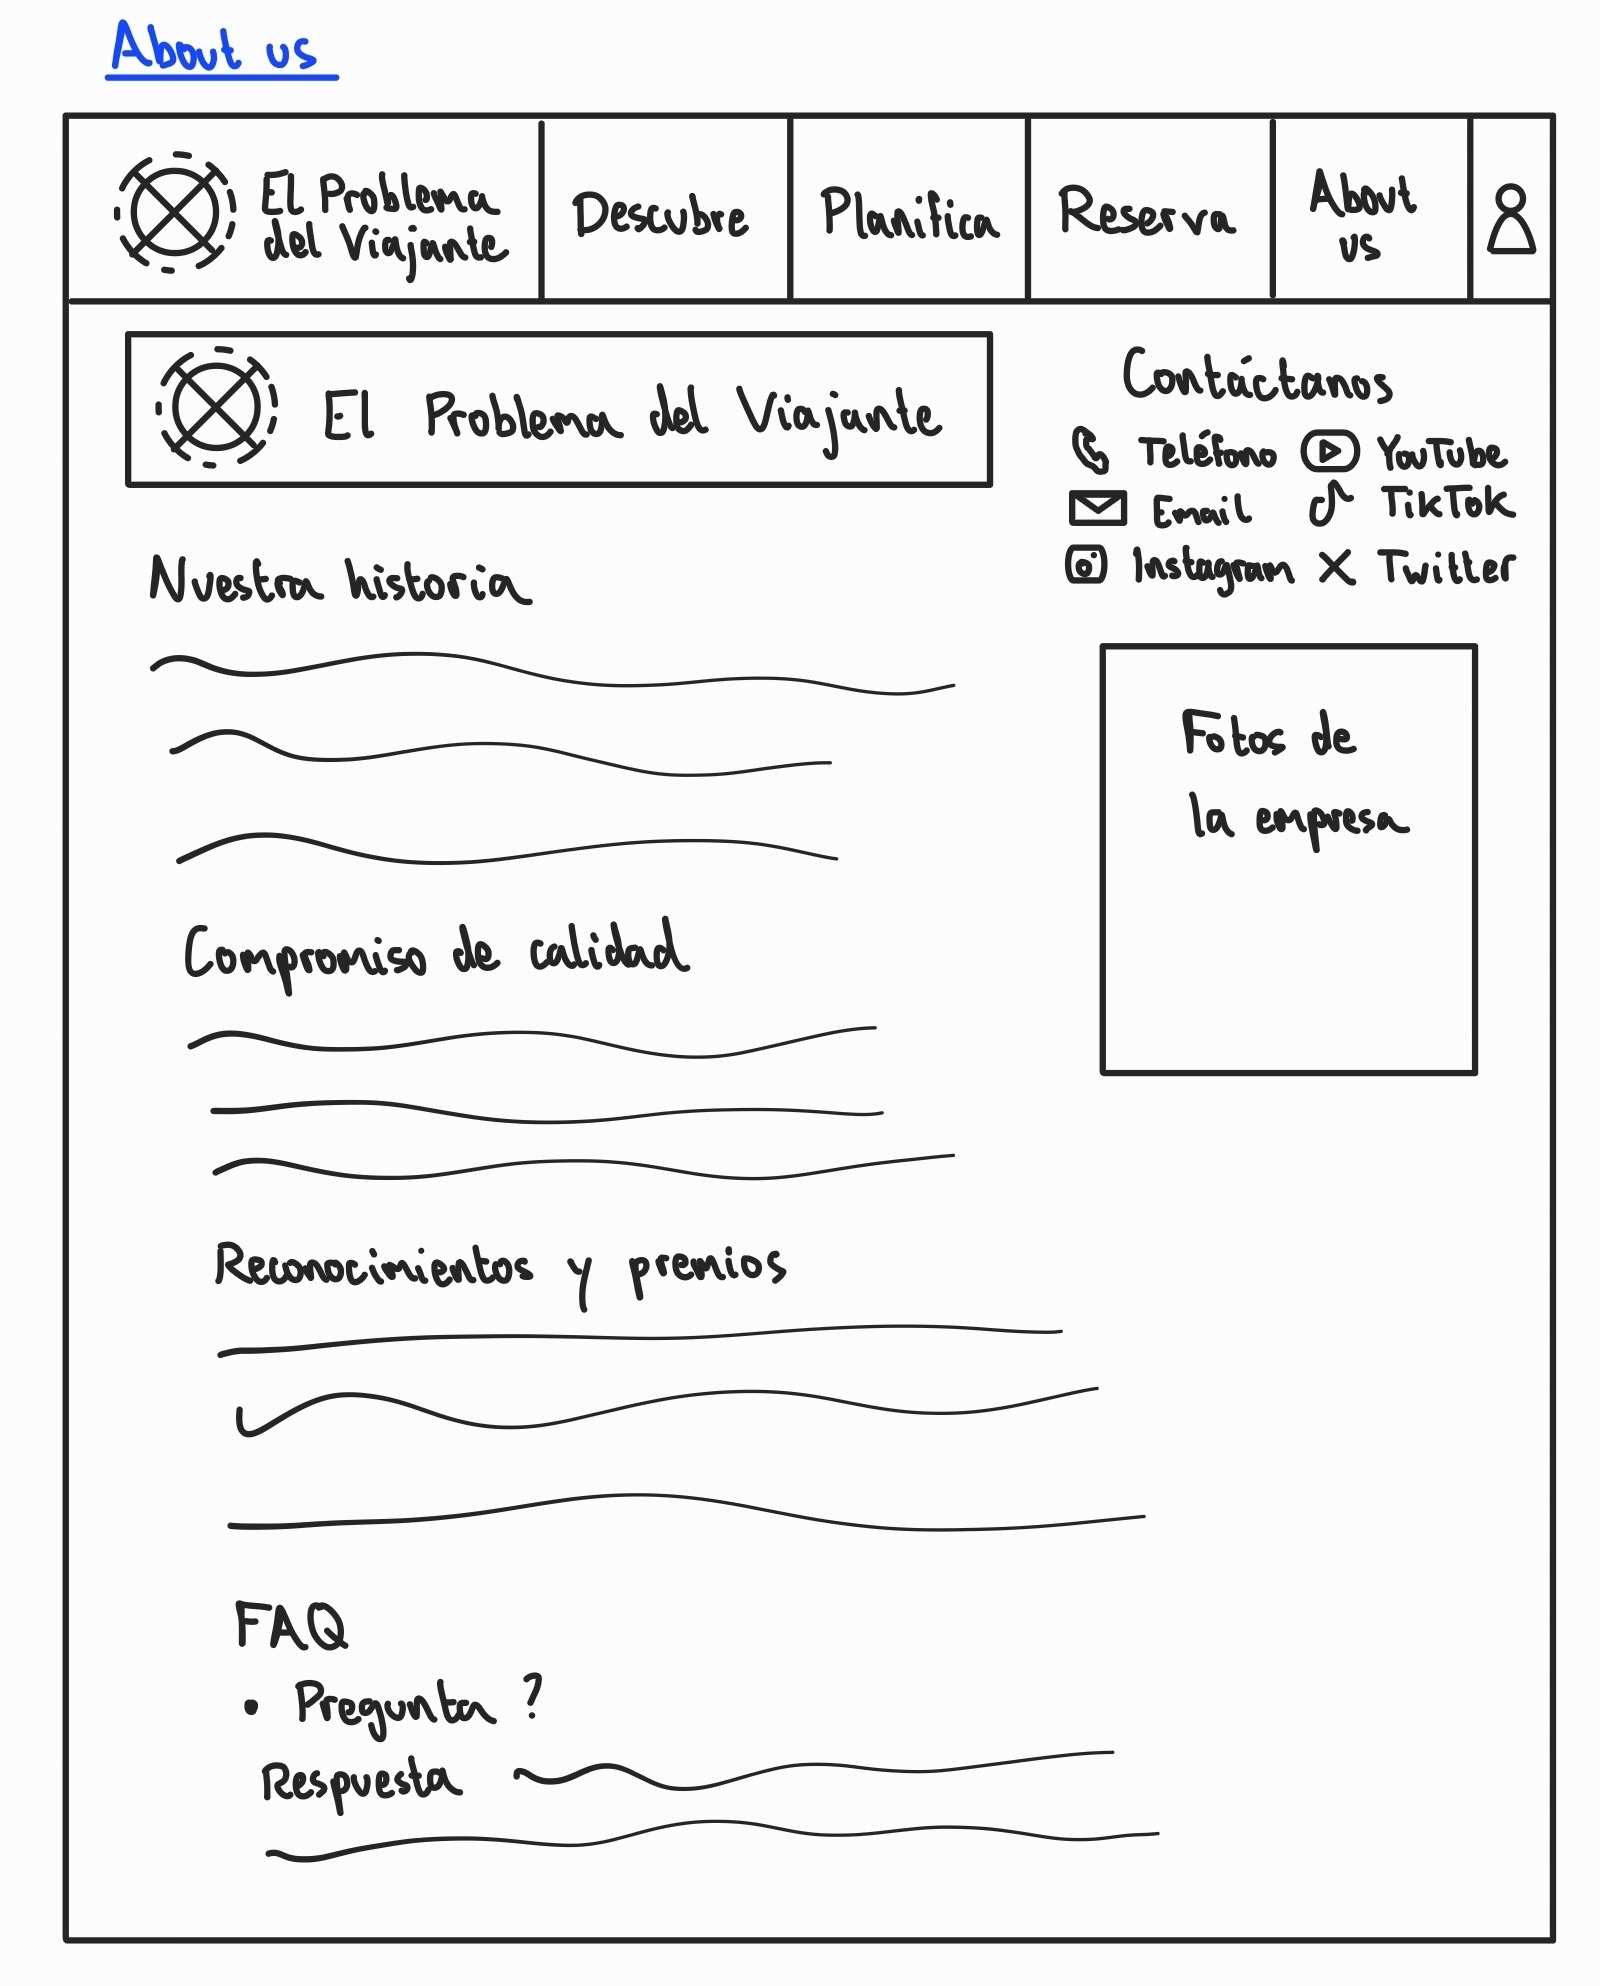
\includegraphics[width=\textwidth]{5-about_us.jpg}
		\caption{Prototipo Página principal}
	\end{figure} 

	La página de \textbf{About us} es principalmente de texto con información sobre la empresa ficticia. Hay información de contacto, la historia de la empresa, reconocimientos y premios, indicadores de calidad y preguntas frecuentes (FAQ).
	
	\newpage
	
	\subsection{Esqueleto digital}
	El \textit{wireframe} ayuda a establecer las proporciones entre los elementos de la página y a establecer la jerarquía de información del documento en términos de tamaño y posición. Para hacer el diseño, se ha utilizado el sitio web \href{https://figma.com}{Figma} está basado en la regla de las 12 columnas, en las que cada una de las páginas se divide verticalmente en 12 partes, el cual es un número suficientemente pequeño para ser fácilmente manejable (a diferencia de trabajar, por ejemplo, empleando píxeles) pero a la vez es lo suficientemente grande y tiene bastantes divisores como para permitir flexibilidad en el diseño. En los diseños que se muestran a continuación se marcan el número de columnas que ocupan los elementos destacados.
	
	Cabe destacar que para crear un diagrama con un tamaño razonable, todos los diagramas empleados se crearon en un tamaño equivalente a la resolución HD estándar (1920x1080 píxeles). Sin embargo, la expectativa de cualquier usuario de un sitio web es que las páginas admitan siempre desplazamiento en vertical para visualizar toda la información de la página. El desplazamiento en horizontal, si bien posible y utilizado, es menos habitual. Por este motivo, se representa el número de columnas pero no el de filas, y muchos de los elementos aparecen artificialmente distorsionados en la horizontal para poder entrar en el tamaño fijado, lo cual no se mantendrá en la página real.
	
	%\newpage
	
	\begin{figure} [H]
		\centering
		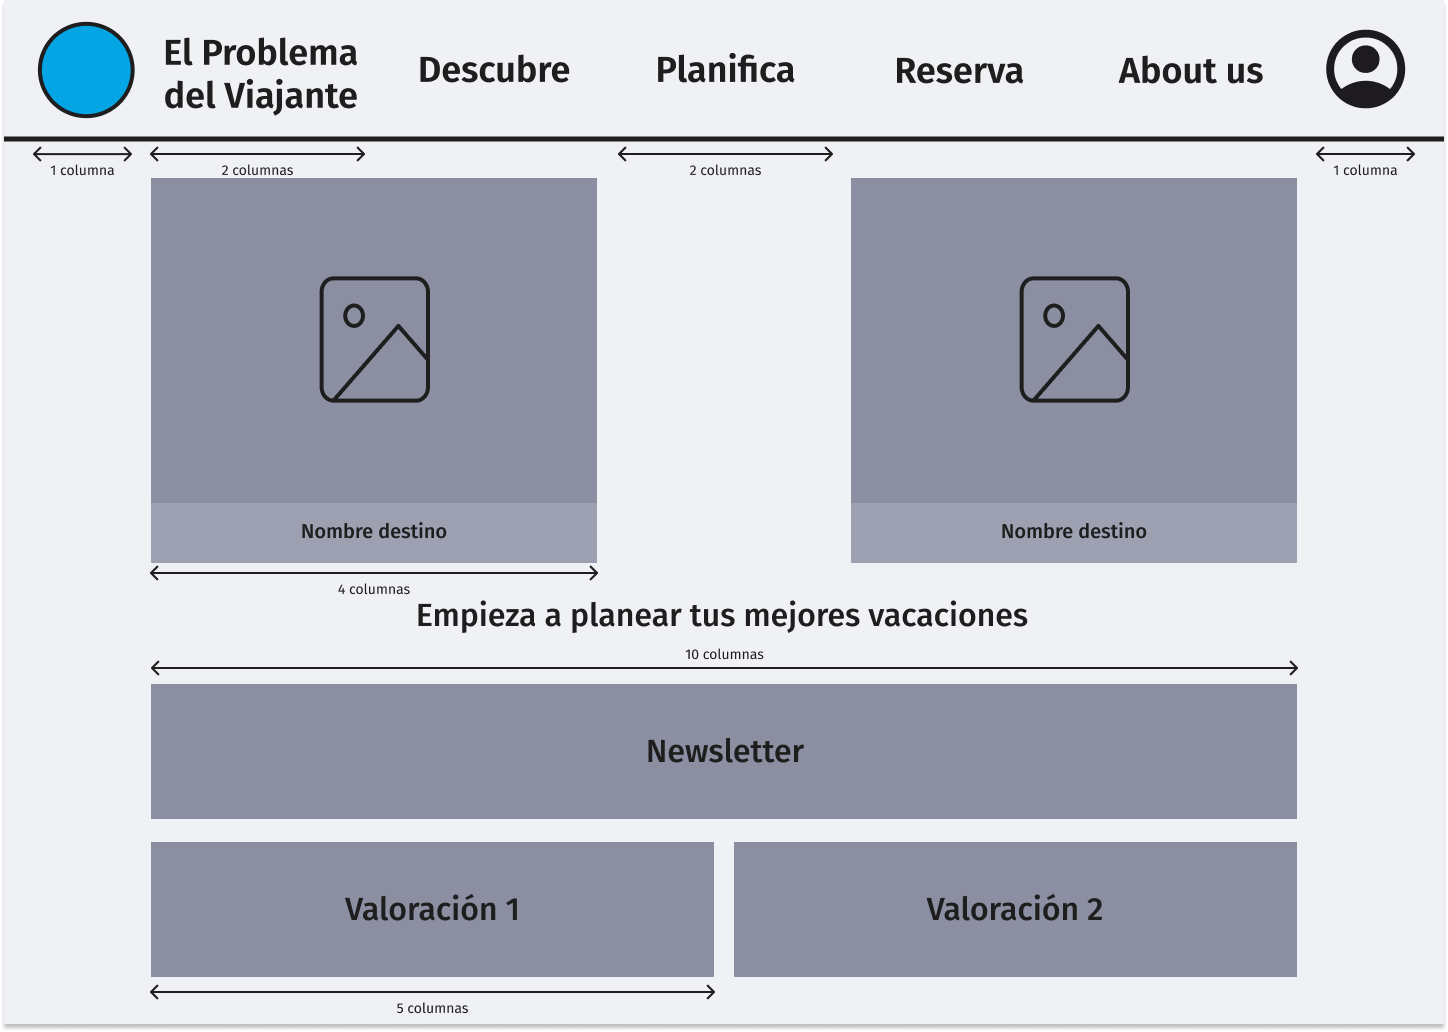
\includegraphics[width=\textwidth]{wireframe-principal.png}
		\caption{Wireframe Página principal}
	\end{figure} 

	Como se ha comentado, se muestran las columnas que ocupa cada elemento. Cabe destacar que la versión final para un dispositivo móvil diferirá significativamente respecto a la imagen mostrada, ya que habrá que tener en cuenta su orientación vertical, por lo que no se mostrarán diseños a dos columnas como este. Por otro lado, el \textit{newsletter} y las valoraciones no se verían completamente al ingresar en la página web, sino que habría que desplazarse verticalmente para visualizar su contenido.
	
	
	\begin{figure} [H]
		\centering
		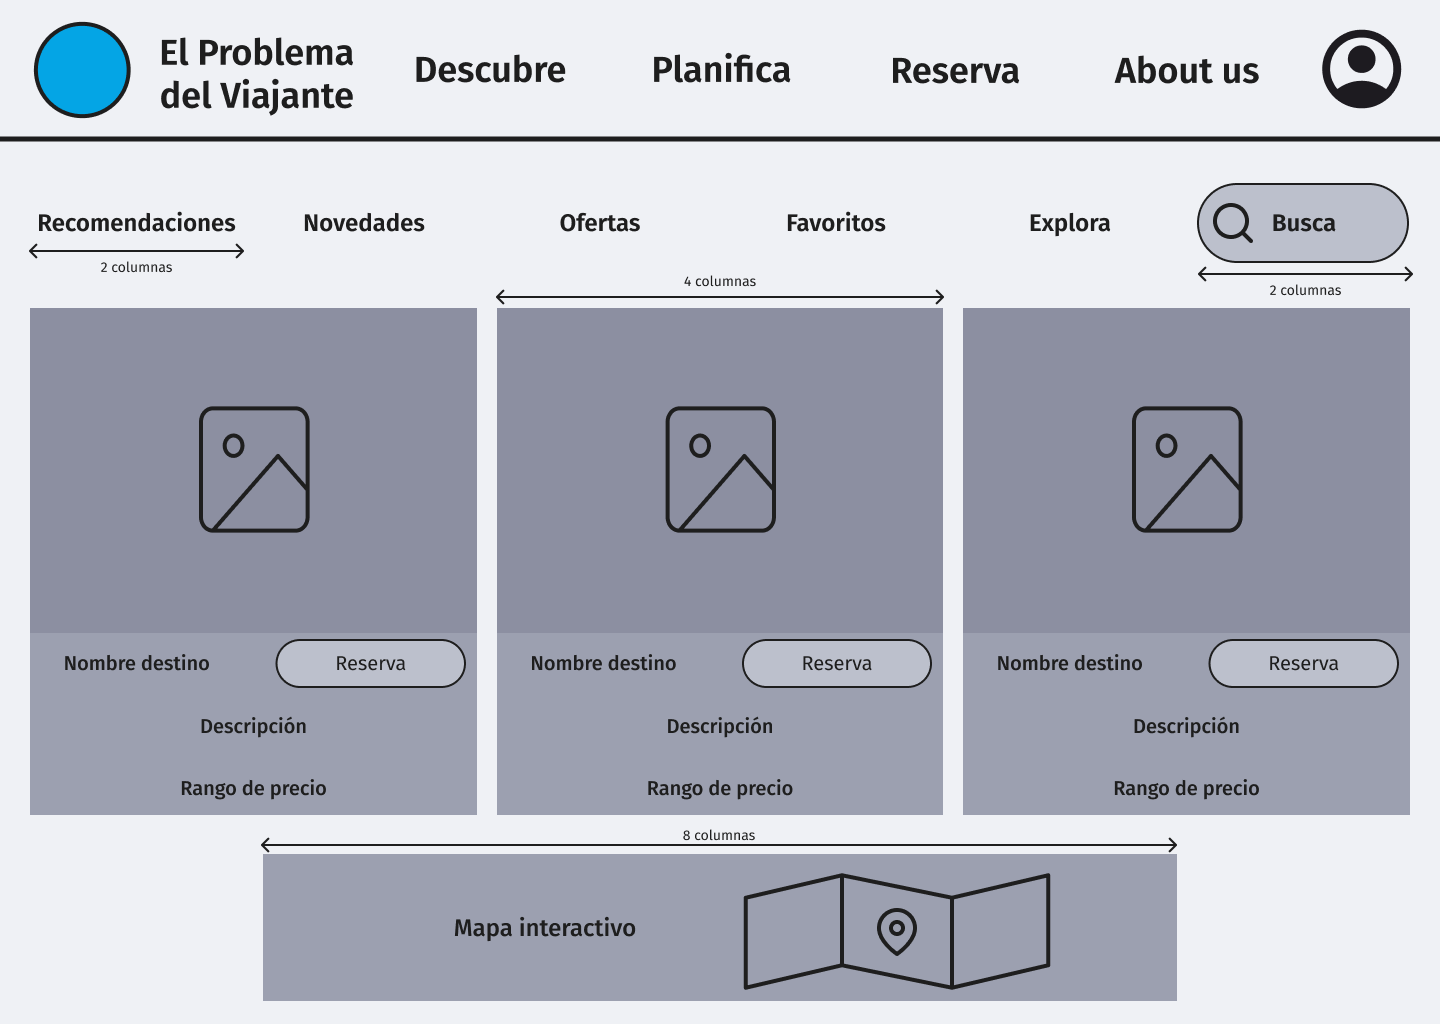
\includegraphics[width=\textwidth]{wireframe-descubre.png}
		\caption{Wireframe Descubre}
	\end{figure}

	En este caso se opta por un diseño a tres columnas, siguiendo la regla de los tercios, en el que las imágenes aparecerían en la parte central de pantalla, y habría una barra de navegación secundario para elegir diferentes formas de búsqueda. De nuevo, en la versión móvil, el diseño sería distinto.
	
	\newpage

	\begin{figure} [H]
		\centering
		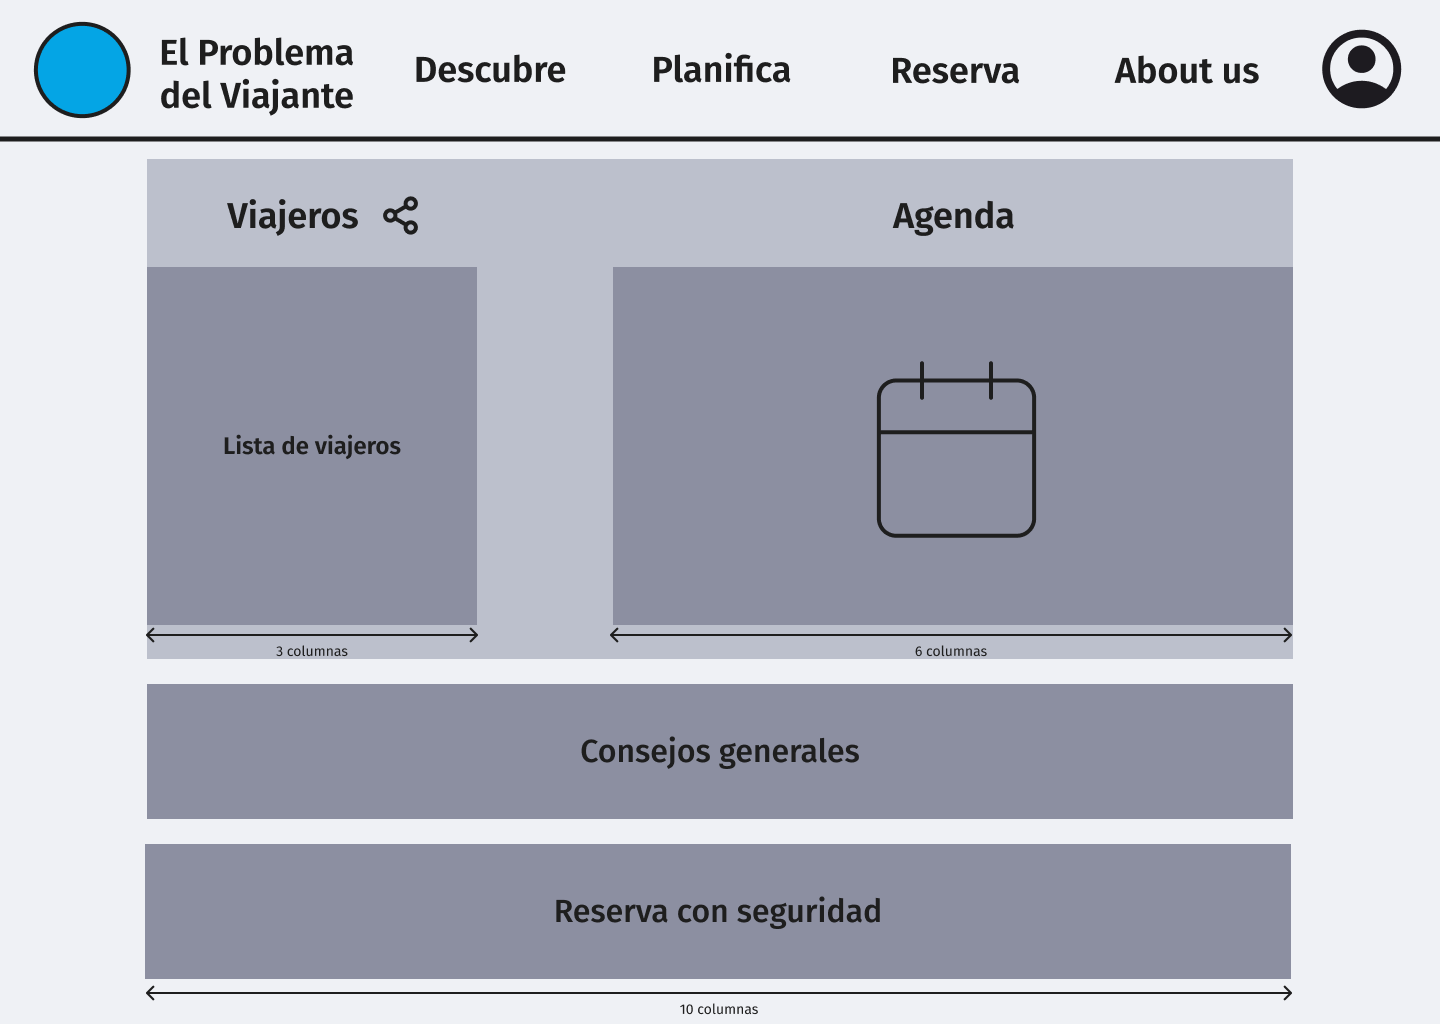
\includegraphics[width=\textwidth]{wireframe-planifica.png}
		\caption{Wireframe Planifica}
	\end{figure}

	En esta pestaña se muestra un calendario compartido por todos los viajeros que estén apuntados a un cierto viaje, junto a las fechas de salida y llegada, los lugares de visita reservados, etc. Más abajo, se encuentran consejos para los viajes, los cuales no se verían completamente en la forma final, ya que ocuparían más espacio del que aparece aquí.

	\newpage
	
	\begin{figure} [H]
		\centering
		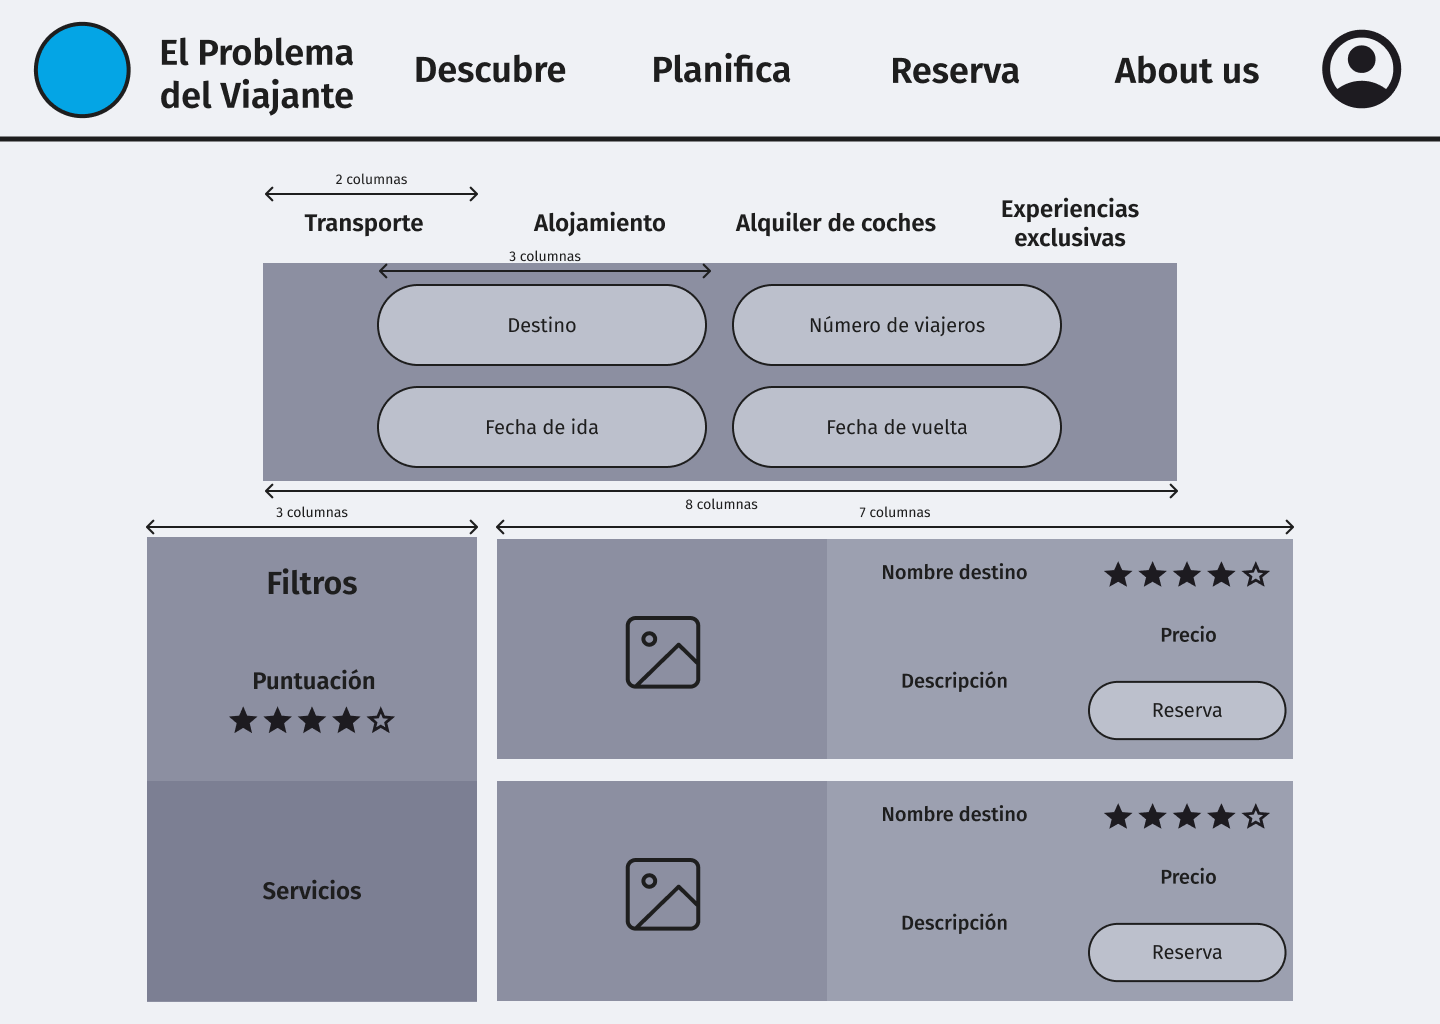
\includegraphics[width=\textwidth]{wireframe-reserva.png}
		\caption{Wireframe Reserva}
	\end{figure}

	En este wireframe se muestra otra barra de navegación secundaria diferente, con las diferentes modalidades de reserva, y múltiples opciones de personalización del viaje, desde la fecha hasta la puntuación y los servicios ofertados. El diseño está inspirado en el de las páginas web de reservas de viajes como \href{https://www.tripadvisor.es/Hotels-g186338-London_England-Hotels.html}{Tripadvisor}.
	
	\newpage
	
	\begin{figure} [H]
		\centering
		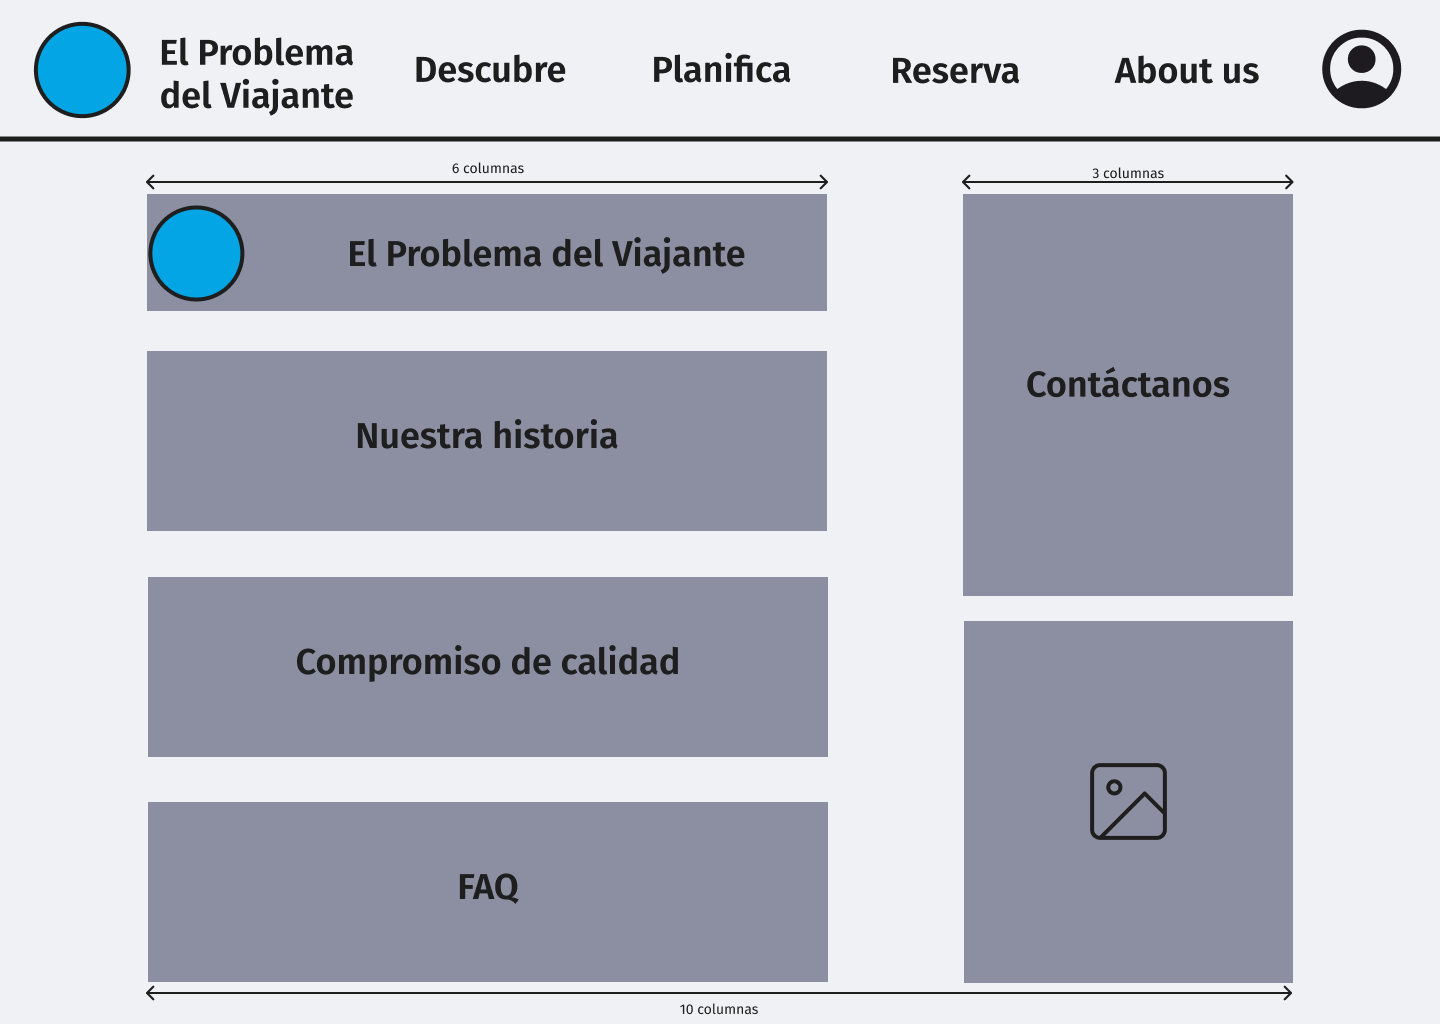
\includegraphics[width=\textwidth]{wireframe-about_us.png}
		\caption{Wireframe About us}
	\end{figure}
	
	Se opta por un diseño con una columna principal con los elementos más relevantes como la historia de la empresa, los indicadores de calidad y las preguntas frecuentes, y una columna secundario con las redes sociales y una imagen de los integrantes de la empresa.
	
	
	
	\subsection{Diseño final}
	El uso de \textit{mockups} permite ver la apariencia final de la página, incluyendo colores, fuentes de texto, logos e imágenes que acompañan al diseño y que hasta este momento se habían obviado. En cuanto la paleta de colores, se optó por usar una paleta ya creada y disponible de forma abierta: \href{https://github.com/catppuccin/catppuccin?tab=readme-ov-file#-palette}{Catppuccin Latte}, a la que se le han añadido algunos colores propios, reutilizados de otros proyectos.
	
	Como tipografía elegida se utilizará Helvetica. Debido a que no está disponible en la herramienta utilizada para el diseño final, se ha usado una letra similar, Fira Sans.
	
	No se añade una descripción a cada una de la imágenes, como se ha hecho en los dos apartados anteriores, ya que muestran la misma disposición del contenido que los \textit{wireframes}, añadiendo los respectivos colores y formateos de texto.
	
	\begin{figure} [H]
		\centering
		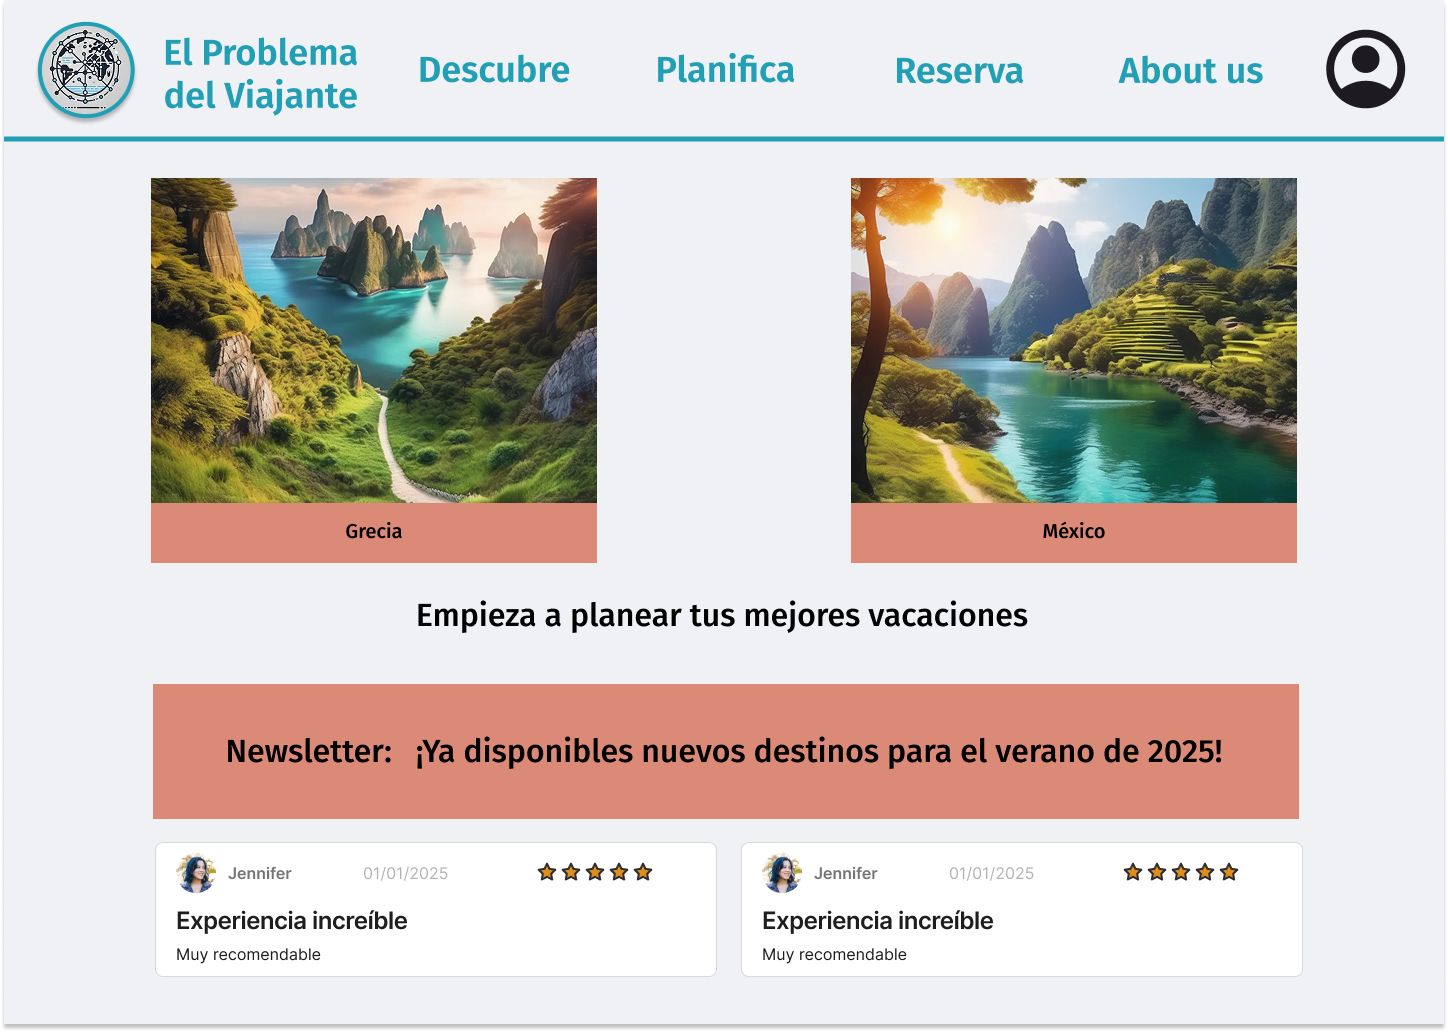
\includegraphics[width=\textwidth]{mockup-principal.png}
		\caption{Mockup Página principal}
	\end{figure}

	\begin{figure} [H]
		\centering
		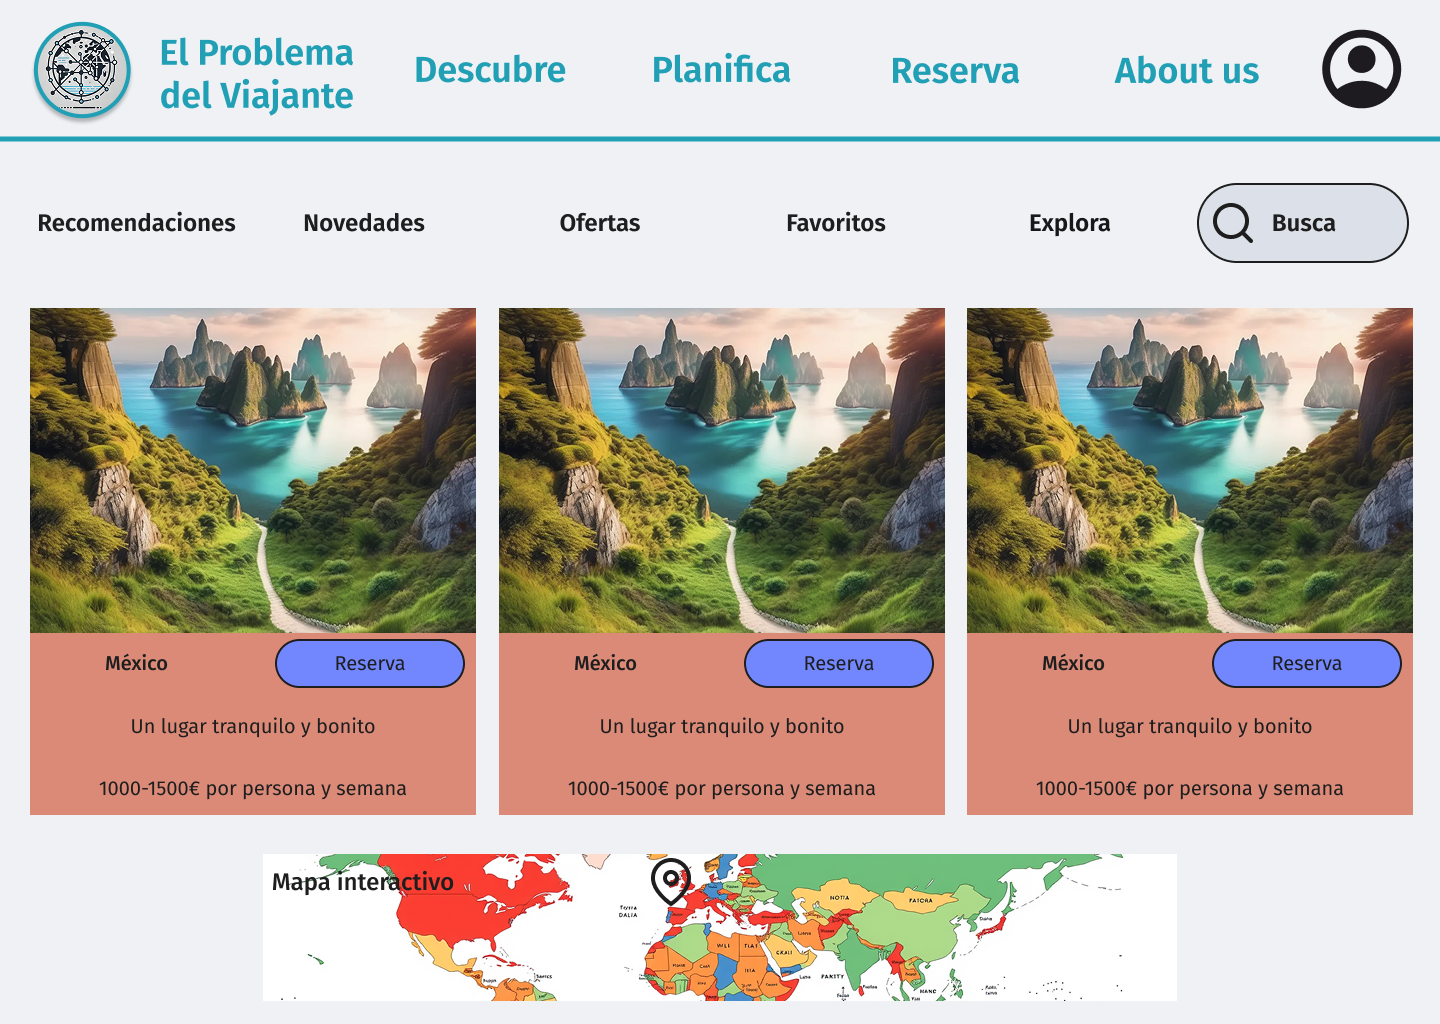
\includegraphics[width=\textwidth]{mockup-descubre.png}
		\caption{Mockup Descubre}
	\end{figure}
	
	\begin{figure} [H]
		\centering
		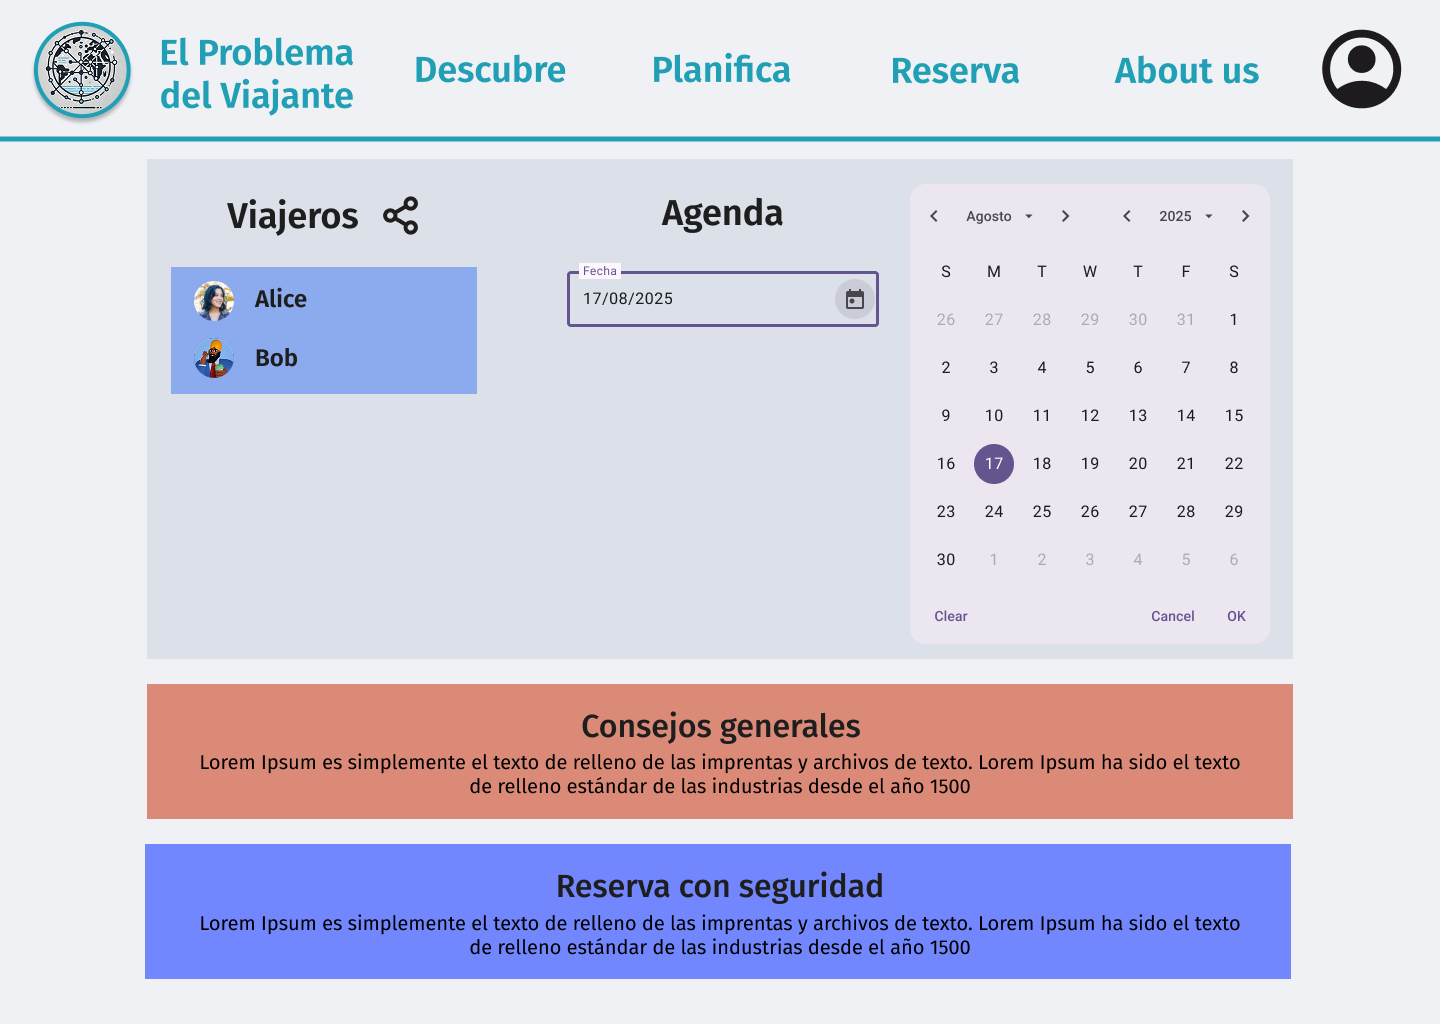
\includegraphics[width=\textwidth]{mockup-planifica.png}
		\caption{Mockup Planifica}
	\end{figure}
	
	\begin{figure} [H]
		\centering
		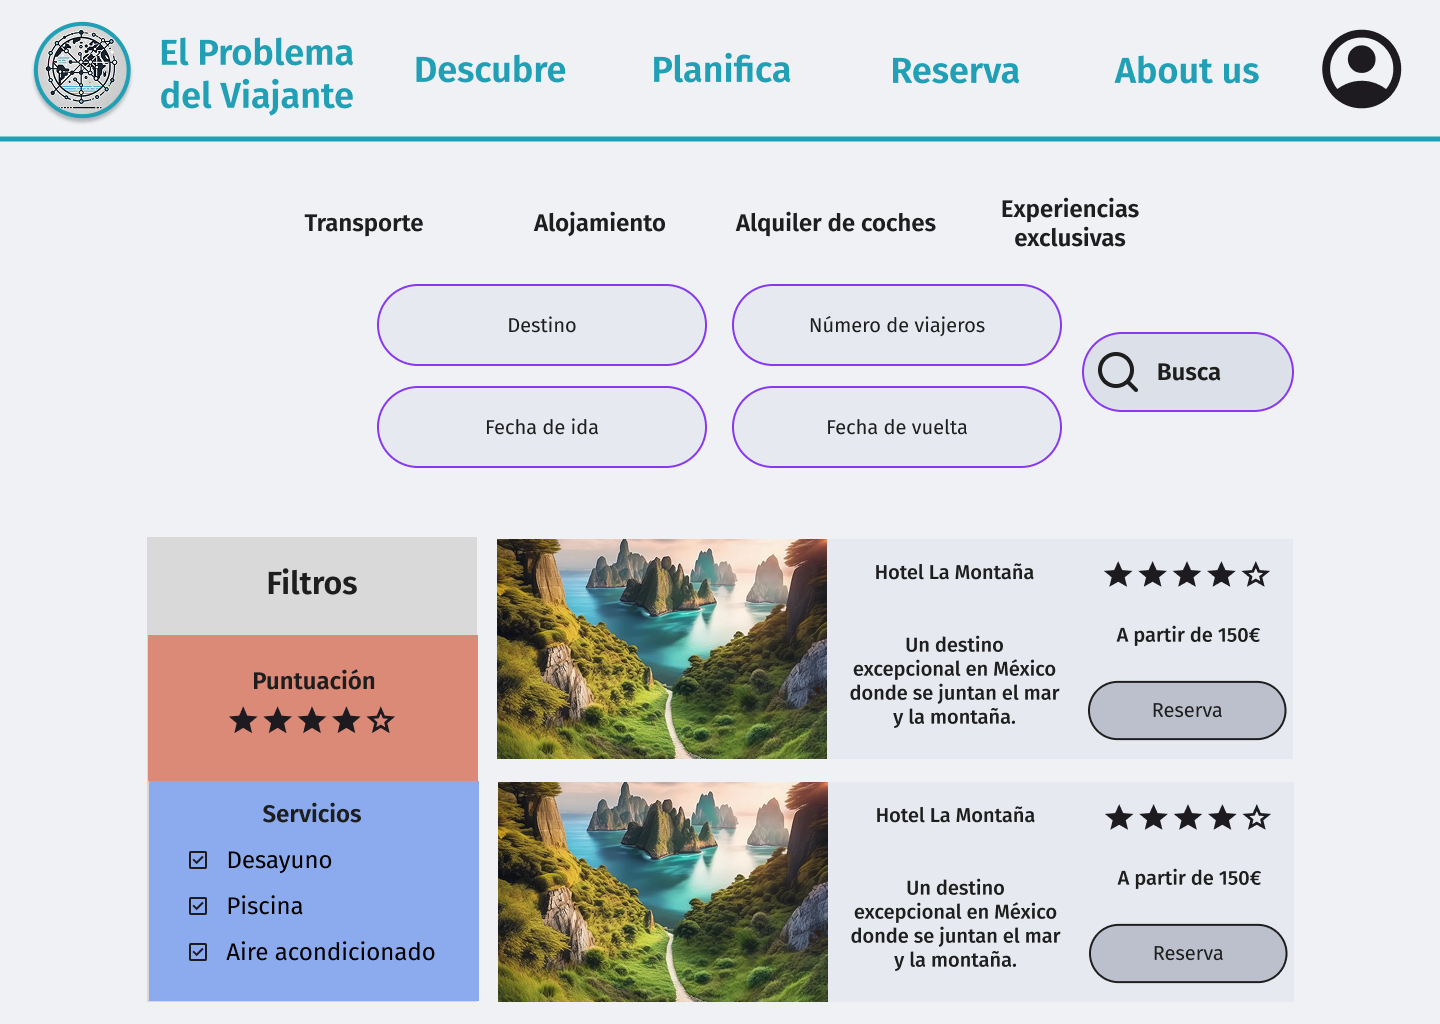
\includegraphics[width=\textwidth]{mockup-reserva.png}
		\caption{Mockup Reserva}
	\end{figure}
	
	\begin{figure} [H]
		\centering
		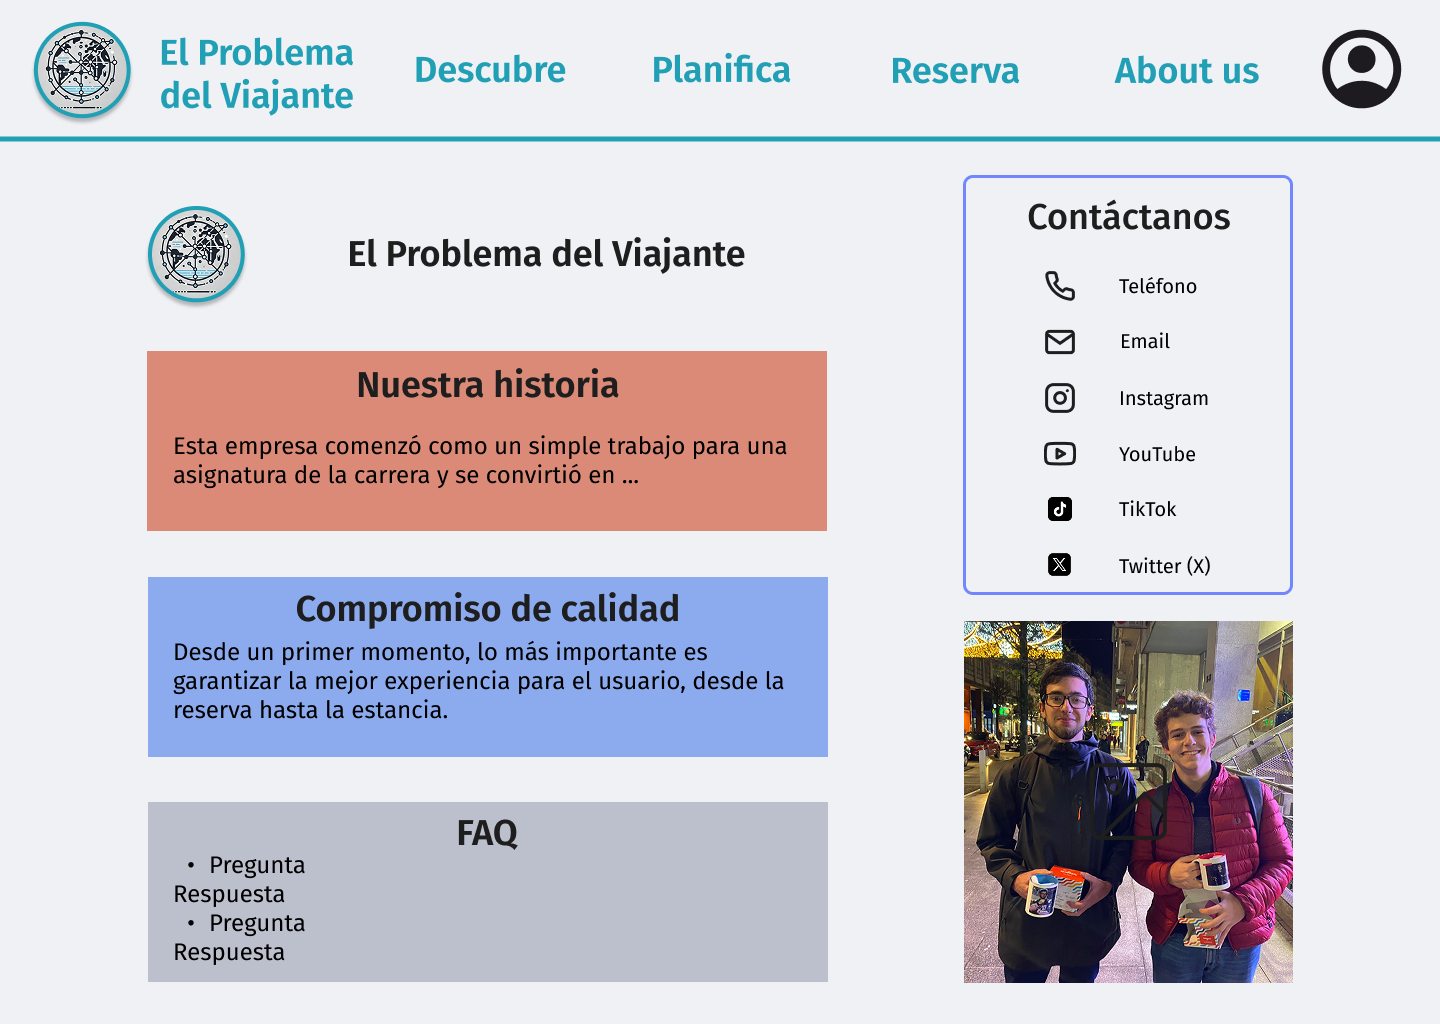
\includegraphics[width=\textwidth]{mockup-about_us.png}
		\caption{Mockup About us}
	\end{figure}


	\newpage
	\section{Storyboard}
	El \textit{storyboard} permite visualizar de forma dinámica el sitio web. Esto permite ilustrar cómo interaccionan elementos y colores, cómo funciona el sistema de navegación propuesto y, en general, tener una idea de si el sitio web representa aquello para lo que fue diseñado.
	
	Para ello, se añade información sobre los diseños finales del apartado anterior, donde se muestra cómo interactuar con los elementos de la página. A continuación se muestran tres casos de uso.
	
	\begin{figure} [H]
		\centering
		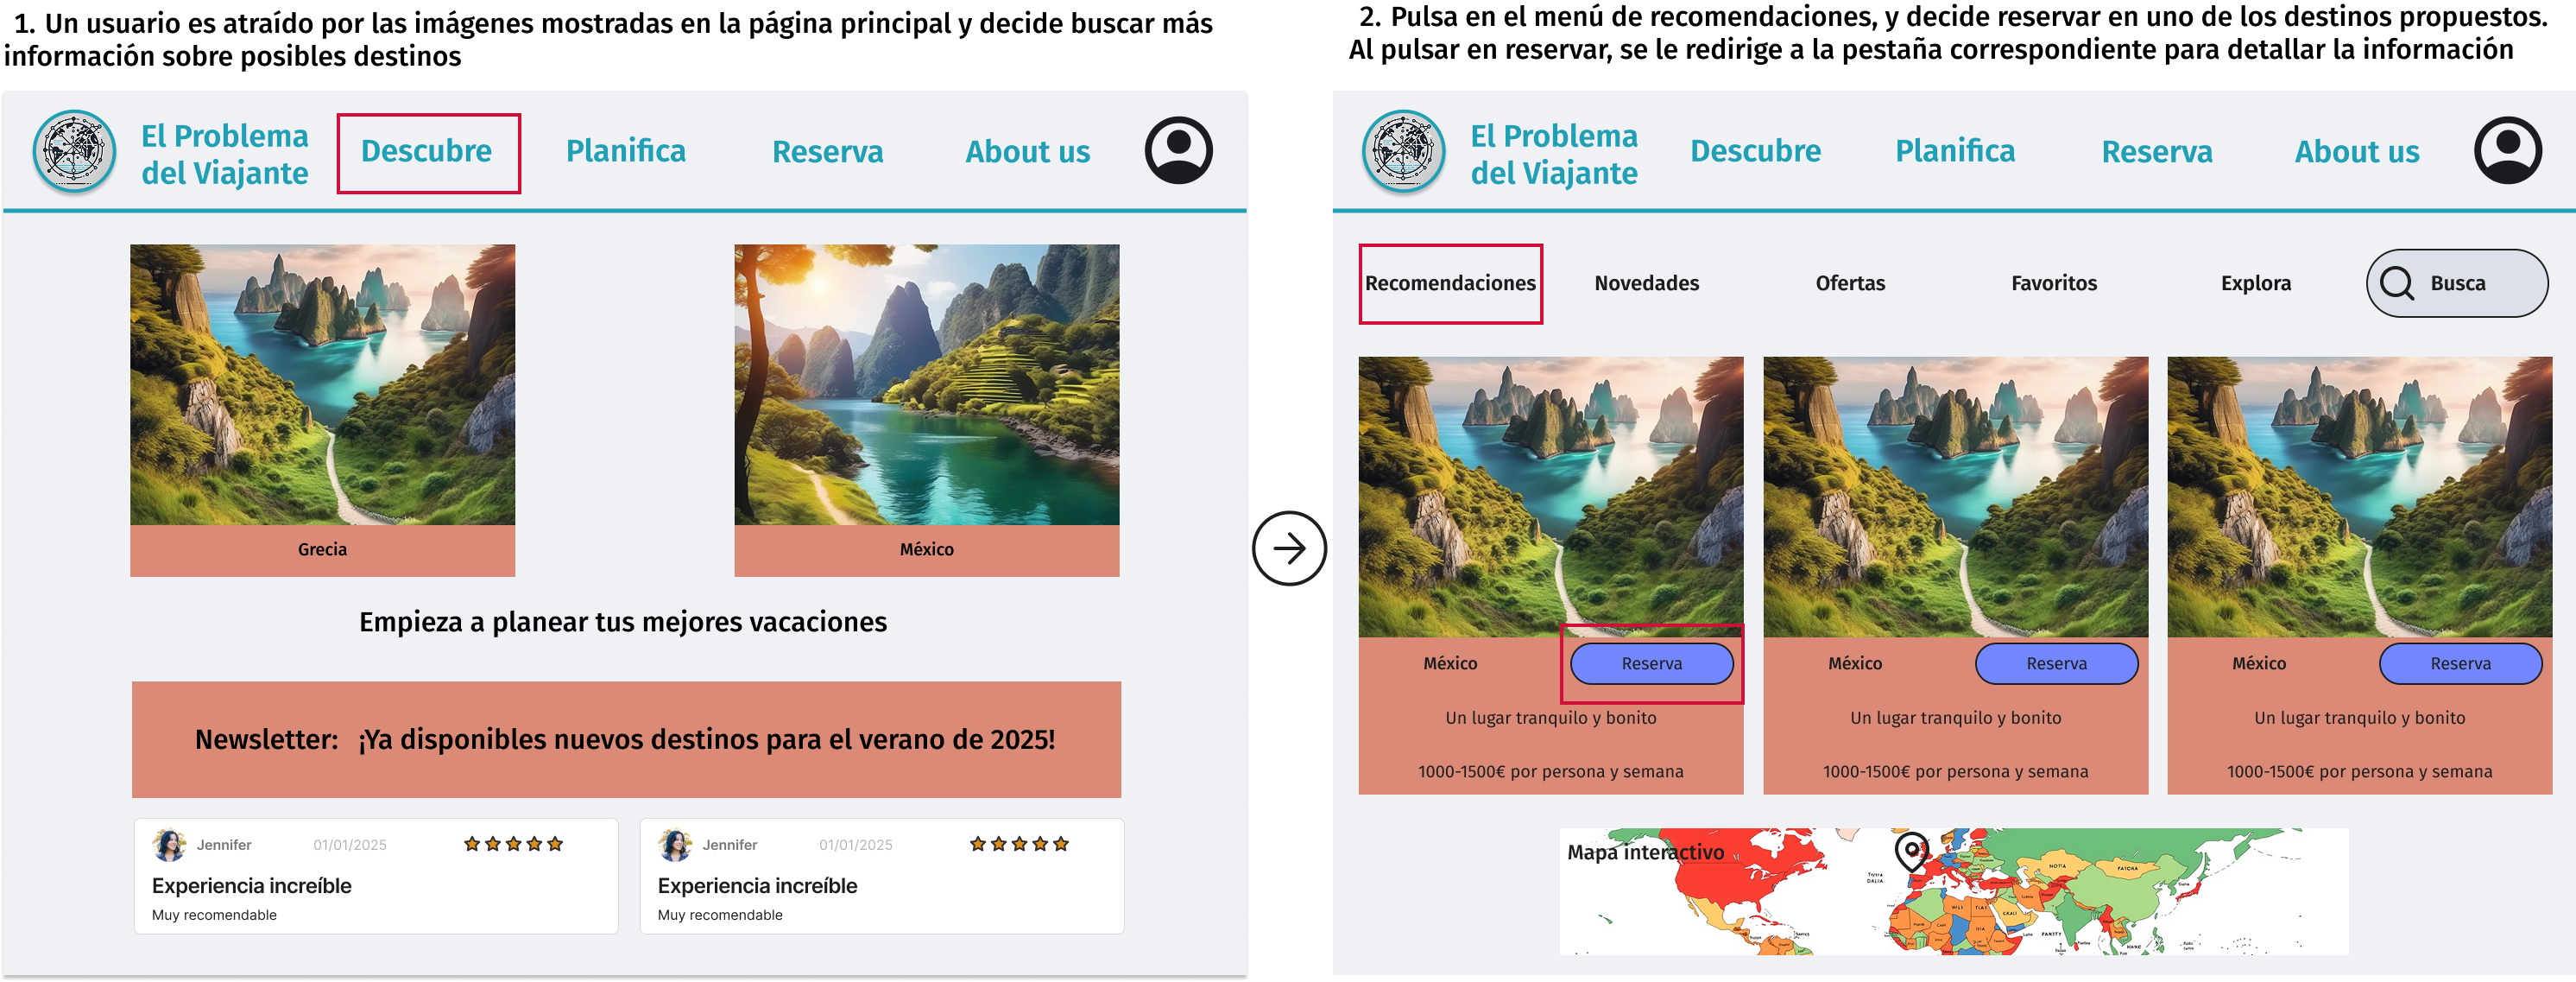
\includegraphics[width=\textwidth]{storyboard-descubrir.png}
		\caption{Storyboard Descubre}
	\end{figure}

	Supongamos que el usuario accede a la página web ya que tiene interés en buscar posibles lugares de visita. Lo intuitivo sería pulsar en la pestaña de \textbf{Descubre} del menú de navegación. En ella, hay diferentes opciones en la barra de navegación secundaria, donde la más relevante sea posiblemente \textbf{Recomendaciones}, y en esta se mostrarán los destinos propuestos. Al pasar el ratón por encima de uno de ellos, el mapa se situará en el lugar donde se encuentran, para facilitar buscar información sobre sus alrededores. Por último, si decidiese que está interesado en hacer la reserva, al pulsar en el correspondiente botón se le redirigiría a la página web desde la que puede reservar.

	\begin{figure} [H]
		\centering
		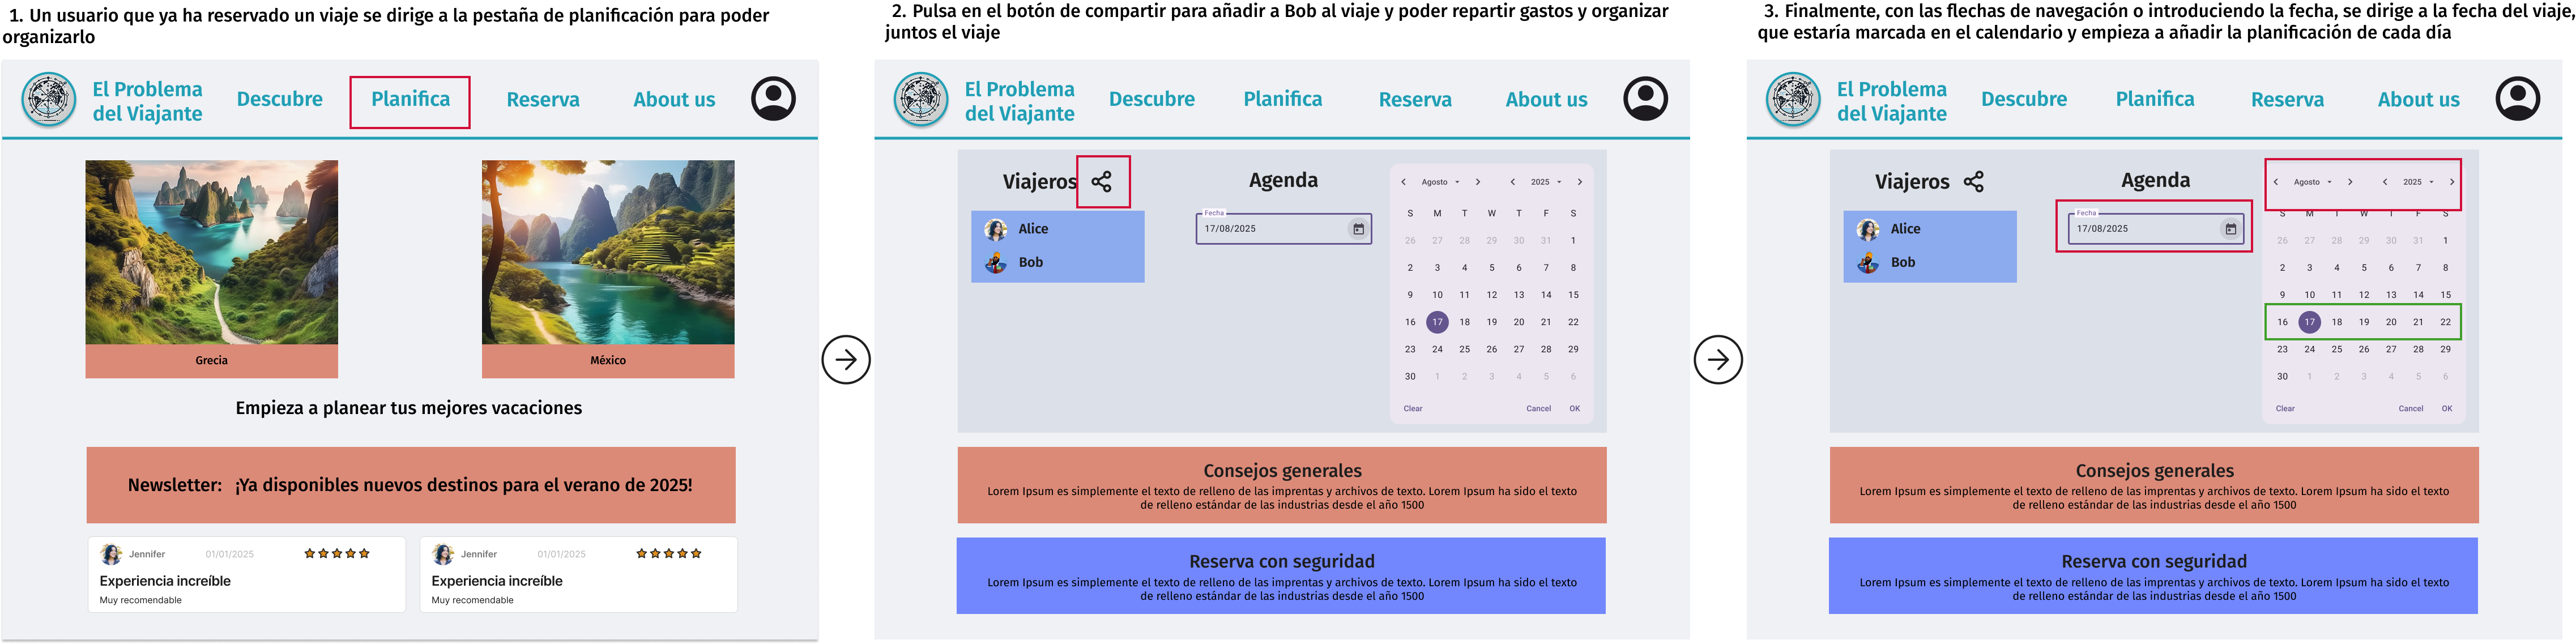
\includegraphics[width=\textwidth]{storyboard-planificar.png}
		\caption{Storyboard Planifica}
	\end{figure}

	\textcolor{red}{La imagen no se ve muy bien, igual hay que pasarla a vertical}
	
	Supongamos ahora que este mismo usuario, tras reservar un viaje y crearse una cuenta en la página web, decide comprobar las fechas de su reserva. Para ello, se dirige a la pestaña de \textbf{Planifica}, desde la que puede añadir a las personas que viajarán con él, lo cual facilita la organización del viaje, la elección de los lugares de visita y el reparto de gastos, además de asegurar que no habrá actividades que se superpongan.
	
	Asimismo, pulsando en el calendario puede cambiar el mes en el que se encuentra y añadir la planificación de cada día según corresponda.
	
	\begin{figure} [H]
		\centering
		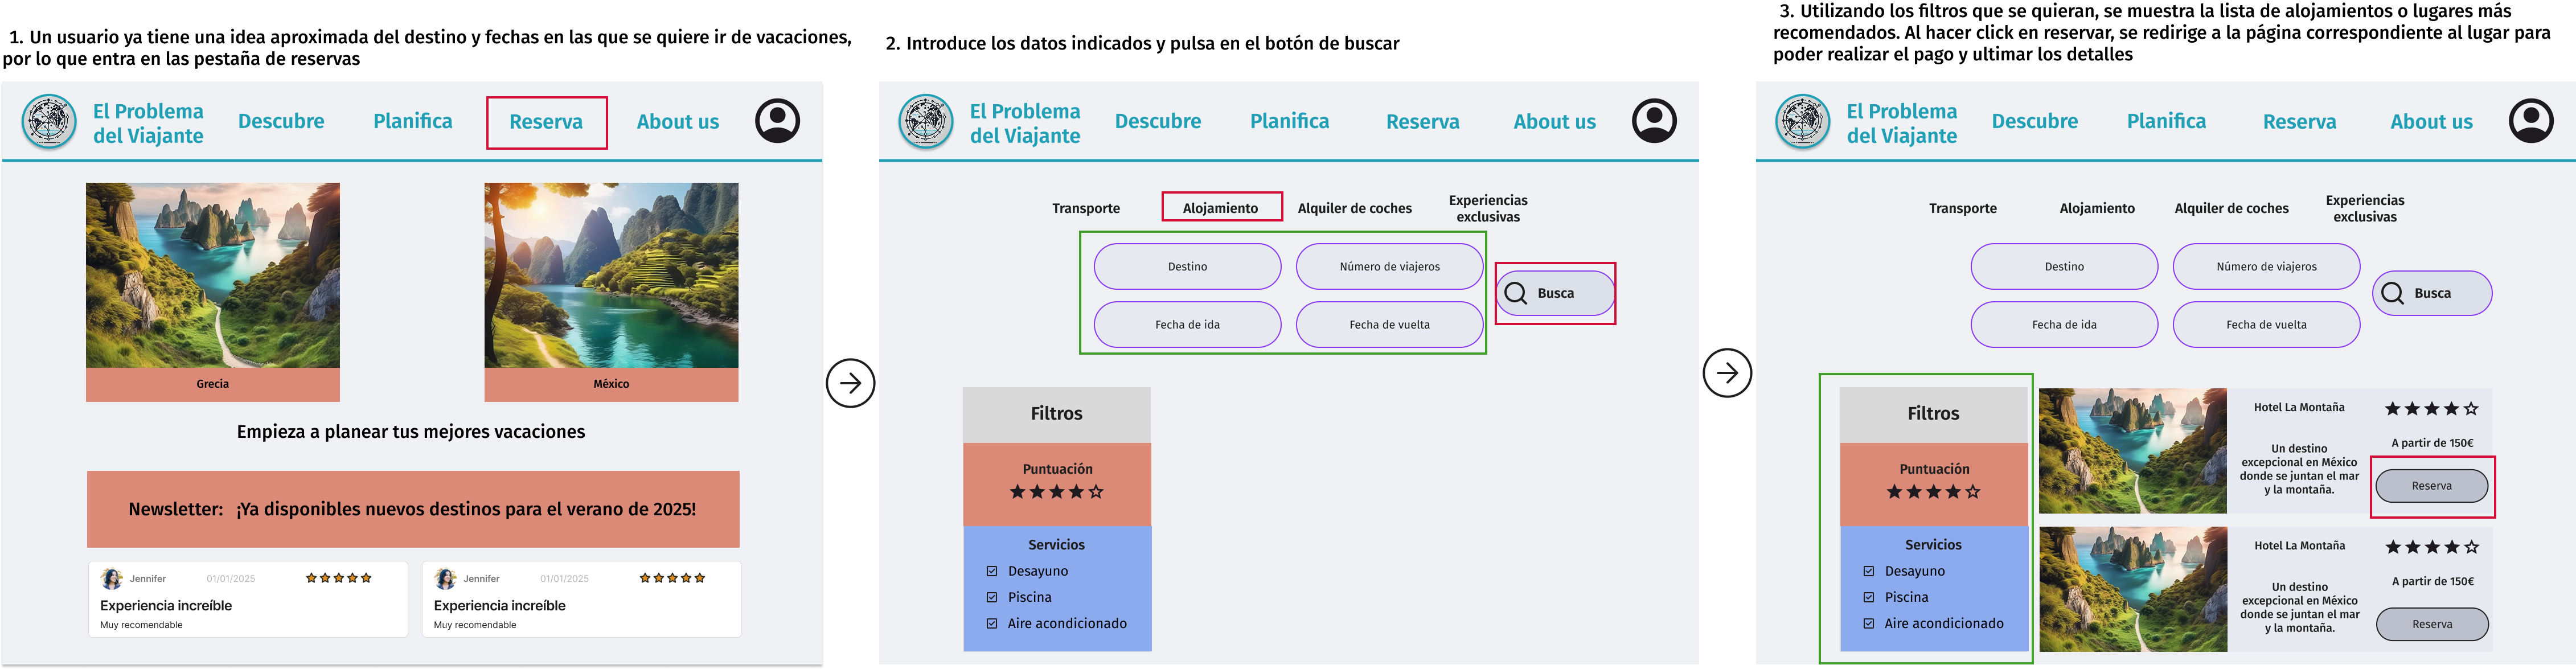
\includegraphics[width=\textwidth]{storyboard-reservar.png}
		\caption{Storyboard Reserva}
	\end{figure}

	Para el último, pensemos en otro usuario que sí tiene claro el destino al que quiere ir, pero no dónde se va a alojar, por lo que accede a la pestaña de \textbf{Reserva}, desde donde podrá ver diferentes ofertas. En la barra de navegación secundaria, selecciona \textbf{Alojamiento} e introduce los datos necesarios, como la fecha ida y de vuelta, y el nombre del destino.
	
	Al pulsar en buscar, se le mostrarán diferentes opciones, ordenadas según los filtro seleccionados, los cuales pueden modificarse para mostrar únicamente alojamientos con una puntuación superior a una dada, o que ofrezcan ciertos servicios como piscina o gimnasio. A continuación, si desea realizar la reserva mostrada, solamente tiene que pulsar en el correspondiente botón, el cual le redirigiría a la página web desde la que puede reservar.


	
	
	
	\section{Estructura de ficheros}
	\label{ficheros}
	Para la organización de los ficheros del proyecto, optamos por una estructura simple en directorios en la que el documento principal, 'index.html', está por sí solo en el nivel raíz, pues es lo que espera el servidor web. 
	
	Por otra parte, tenemos un directorio con la documentación en el que se incluye este documento y sus imágenes asociadas en su correspondiente subdirectorio, así como otros elementos de documentación que puedan surgir en el futuro.
	
	Para los contenidos en sí de la página web, disponemos de cuatro subdirectorios. Uno está destinado a almacenar todas las imágenes que serán necesarias para la elaboración del sitio web. Por otra parte, disponemos de una carpeta en la que se almacenarán los documentos HTML que darán estructura a las diferentes páginas. En el directorio de estilos se almacenarán los ficheros de CSS necesarios para dotar al sitio web de una apariencia profesional y consistente. Por último en el directorio de scripts se incluirán los ficheros de JavaScript que doten al sitio web de funcionalidades dinámicas. 
	
	\begin{figure} [H]
		\centering
		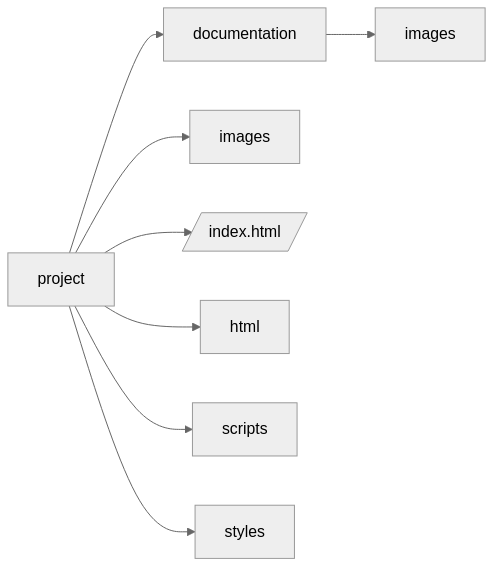
\includegraphics[width=0.8\textwidth]{estructura_ficheros.png}
		\caption{Diagrama de la estructura de ficheros}
	\end{figure}
	
	
	
	
	
	
	
	
	
	% ----------------------------------------------------------------------------
	% ----------------------------------------------------------------------------
	
	\chapter{Documentación HTML}
	
	En la siguiente parte del proyecto, se empieza a codificar el código HTML de las páginas, centrándose en el uso adecuado de las etiquetas HTML, siguiendo los estándares de \href{https://html.spec.whatwg.org/multipage/}{W3C}, y de momento no se codifican características de visualización de la página, pues corresponden a la parte de hojas de estilo. 
	
	Para cada una de las cinco página principales, se muestra a continuación su mapa de etiquetas.
	
	\begin{Huge}
		\textcolor{red}{Ojo que faltan algunos por hacer}
	\end{Huge}
	
	La mayoría de las otras páginas de la web son muy semejantes a las mostradas (por ejemplo, en las que tienen un menú de navegación secundario, las diferencias entre sí son ínfimas), y otras como la pestaña de Política de privacidad o Términos y condiciones solamente tienen contenido de texto a una columna, por lo que no aporta información mostrar su mapa de etiquetas.
	
	
	
	
	
	
	% ----------------------------------------------------------------------------
	% ----------------------------------------------------------------------------
	
	\chapter{Documentación CSS}
	
	\textcolor{red}{Para cada efecto hay que hacer un diagrama con los ids usados y mostrando el efecto con dos/tres pantallazos. Como falta retocar, aun no hago nada de esto}
	
	Página principal: Bootstrap, posible carrusel
	Descubre: Multicol
	Planifica: CSS Grid
	Reserva: Flex, filas para abajo
	About us: Flexible Grids
	
	\section{Flexible Grids}
	\section{CSS Multicol}
	\section{Flex Container}
	\section{CSS Grid}
	\section{Bootstrap}
	

	
	
	
	
	
	
	\chapter{Documentación JavaScript}
	
	\textcolor{red}{Pero como voy a documentar código con capturas de pantalla}
	
	JavaScript
	Semana 1: refactor menú navegación, calendario de Planifica
	Semana 2: quizás se pueda añadir JQuery a algo de la semana 1
	
	\section{Acceso al DOM}
	
	\section{Uso de jQuery y JES6}
	
	\section{Carga de contenido}
	
	
	
	
	
	\chapter{Anexo}
	\label{chap:anexo1}
	\section{Tormenta de ideas}
	
	Todos los elementos obtenidos durante la tormenta de ideas son:
	
	\begin{itemize}
		\item Presentación de la página
		\item Destinos de moda/recomendados
		\item Exploración (lugares menos conocidos, o aleatorios)
		\item About us: quiénes somos, nuestra historia, qué nos diferencia
		\item Búsqueda de hoteles
		\item Búsqueda de medios de transporte (avión, tren, autobús, etc.)
		\item Lugares de visita, ocio, restauración, etc.
		\item Alquiler de coches
		\item Experiencias exclusivas
		\item Calendario para la planificación del viaje
		\item Mapa de lugares favoritos
		\item Newsletter con novedades
		\item FAQ
		\item Mecanismos de reserva con seguridad
		\item Seguro de viajes
		\item Consejos generales para viajes al extranjero
		\item Nuestro sistema de puntuación
		\item Opiniones de expertos
		\item Certificados de calidad, premios
		\item Redes sociales
		\item Términos de uso, política de cookies, política de privacidad
	\end{itemize}


	\section{Cambios}
	\label{sect:anexo2}
	En esta sección se incluye una lista de cambios realizados a lo largo del proyecto, que difieren respecto al diseño original que se planteó. Cada uno incluye una breve descripción y una justificación de por qué se ha hecho.
	
	\subsection{Diseño final}
	\textcolor{red}{------------------------ Hay que escribir esto bien y razonar -----------------------}
	Principal: se ha cambiado la zona principal por un carrusel con bootstrap
	About us: se han cambiado los recuadros de colores por solo los bordes de colores, para no saturar demasiado
	Planifica: lo mismo
	
	
	\subsection{Estructura de ficheros}
	La estructura de ficheros general se ha mantenido a lo largo del proyecto, aunque se ha añadido algún subdirectorio a los que se mencionan en \ref{ficheros}. Concretamente, cada una de las cinco páginas principales tiene su propio directorio dentro de /html y /images, con el objetivo de facilitar la gestión de grandes cantidades de contenido.
	
	
	
	\begin{thebibliography}{widestlabel}
		\href{https://html.spec.whatwg.org/multipage/}{W3C}
		Aquí deberían ir páginas de consulta (w3schools, bootstrap, flatpickr, etc.), y quizás páginas en las que nos hemos inspirado
	\end{thebibliography}
	
	
	
\end{document}